% ============================================================
% HSBI Beamer — ISLP Lecture Series — IMPROVED EDITION
% Chapter 4: Classification
% ============================================================
\documentclass[aspectratio=169,11pt]{beamer}
\usepackage[utf8]{inputenc}\usepackage[T1]{fontenc}\usepackage[english]{babel}
\usepackage{graphicx}\usepackage{booktabs}\usepackage{amsmath,amssymb,amsfonts}
\usepackage{mathtools}\usepackage{hyperref}\usepackage{xcolor}
\usepackage{verbatim}\usepackage{alltt}
\usepackage{tikz}\usetikzlibrary{calc,arrows.meta,positioning,shapes}
\usepackage{tcolorbox}\tcbuselibrary{skins}

\usetheme{Madrid}\usecolortheme{default}
\setbeamertemplate{navigation symbols}{}
\setbeamertemplate{footline}[frame number]
\setbeamertemplate{blocks}[rounded][shadow=false]
\setbeamertemplate{headline}{%
  \leavevmode\hbox{%
    \begin{beamercolorbox}[wd=\paperwidth,ht=2.2ex,dp=0.9ex]{section in head/foot}%
      {\fontsize{4.6}{5.2}\selectfont%
       \insertsectionnavigationhorizontal{\paperwidth}{}{\hskip0pt plus1filll}}%
    \end{beamercolorbox}}%
}
\setbeamerfont{section in head/foot}{size=\tiny}
\setbeamerfont{palette primary}{size=\tiny}
\setbeamerfont{palette tertiary}{size=\tiny}
\setbeamerfont{section in toc}{size=\footnotesize}

\usepackage{listings}
\definecolor{pyKw}{RGB}{0,0,180}\definecolor{pyStr}{RGB}{20,120,40}
\definecolor{pyCom}{RGB}{120,120,120}\definecolor{accent}{RGB}{38,70,140}
\lstdefinestyle{Pystyle}{language=Python,basicstyle=\ttfamily\footnotesize,
  keywordstyle=\color{pyKw}\bfseries,commentstyle=\color{pyCom}\itshape,
  stringstyle=\color{pyStr},showstringspaces=false,upquote=true,
  columns=fullflexible,breaklines=true,literate={~}{{$\sim$}}1}
\lstset{style=Pystyle}

\usepackage{etoolbox}
\makeatletter
\patchcmd{\beamer@sectionintoc}{\vskip1.5em}{\vskip.6em}{\typeout{TOCPATCH-OK}}{\typeout{TOCPATCH-FAIL}}
\makeatother

\AtBeginSection[]{\begin{frame}{Outline}\scriptsize
  \tableofcontents[currentsection,sectionstyle=show/shaded,subsectionstyle=show/show/hide]
\end{frame}}

\newcommand{\islpsource}[1]{%
  \vfill\hfill{\tiny\itshape\color{gray}Source: #1 \textemdash{} ISLP, James et al.\ (2023).}\par
}

\newtcolorbox{takeaway}[1][Takeaway]{enhanced,colback=green!4,colframe=green!50!black,
  boxrule=0pt,leftrule=2.5pt,arc=2pt,fonttitle=\bfseries,title=#1,
  left=2mm,right=2mm,top=1mm,bottom=1mm}
\newtcolorbox{numexample}[1][Worked example]{enhanced,colback=orange!4,colframe=orange!70!black,
  boxrule=0pt,leftrule=2.5pt,arc=2pt,fonttitle=\bfseries,title=#1,
  left=2mm,right=2mm,top=1mm,bottom=1mm}
\newtcolorbox{readme}[1][How to read this]{enhanced,colback=blue!4,colframe=accent,
  boxrule=0pt,leftrule=2.5pt,arc=2pt,fonttitle=\bfseries,title=#1,
  left=2mm,right=2mm,top=1mm,bottom=1mm}

\title{Quantitative Research Methods}
\subtitle{Chapter 4: Classification}
\author{Prof.\ Dr.\ Christoph Weisser}\institute{HSBI}
\date{Summer Semester 2026}\graphicspath{{images/}}

\newtcolorbox{exercise}[1][Exercise]{enhanced, fontupper=\footnotesize, colback=purple!4, colframe=purple!55!black, boxrule=0pt, leftrule=2.5pt, arc=2pt, fonttitle=\bfseries, title=#1, left=2mm, right=2mm, top=1mm, bottom=1mm}
\newtcolorbox{solutionbox}[1][Solution]{enhanced, fontupper=\footnotesize, colback=teal!5, colframe=teal!55!black, boxrule=0pt, leftrule=2.5pt, arc=2pt, fonttitle=\bfseries, title=#1, left=2mm, right=2mm, top=1mm, bottom=1mm}
\newtcolorbox{longexercise}[1][Extended exercise (15 min)]{enhanced, fontupper=\footnotesize, colback=violet!6, colframe=violet!55!black, boxrule=0pt, leftrule=3pt, arc=2pt, fonttitle=\bfseries, title=#1, left=2mm, right=2mm, top=1mm, bottom=1mm}

% Reclaim ~2pt of body height (custom nav headline makes full slides tip over by ~1.83pt)
\addtobeamertemplate{frametitle}{}{\vspace{-2pt}}

\newtcolorbox{labnote}[1][Run this live in the lab notebook]{enhanced, fontupper=\footnotesize, colback=cyan!7, colframe=cyan!45!black, boxrule=0pt, leftrule=3pt, arc=2pt, fonttitle=\bfseries, title=#1, left=2mm, right=2mm, top=1mm, bottom=1mm}

\begin{document}
\begin{frame}[plain]\titlepage\end{frame}

\begin{frame}{The course at a glance}
  \footnotesize
  \begin{center}
  \begin{tabular}{@{}c r l@{}}
    & \textbf{Lecture} & \textbf{Topic}\\
    \midrule
     & 1 & Ch.\ 1 + 2 --- Introduction; what is statistical learning \\
     & 2 & Ch.\ 2 --- Accuracy, bias--variance, Bayes classifier, KNN \\
     & 3--4 & Ch.\ 3 --- Linear regression (estimation, inference, diagnostics) \\
    $\blacktriangleright$ & \textbf{5--6} & \textbf{Ch.\ 4 --- Classification (logistic, LDA/QDA, naive Bayes, ROC)} \\
     & 7 & Ch.\ 5 --- Resampling (validation, CV, bootstrap) \\
     & 8 & Ch.\ 6 --- Model selection and regularisation (ridge, lasso) \\
     & 9 & Ch.\ 7 --- Moving beyond linearity (splines, GAMs) \\
     & 10 & Ch.\ 8 --- Tree-based methods (trees, forests, boosting) \\
     & 11 & Ch.\ 10 --- Deep learning (MLPs, CNNs, training) \\
     & 12 & Ch.\ 13 --- Multiple testing (FWER, FDR) \\
  \end{tabular}
  \end{center}
  \vspace{2pt}
  {\scriptsize Twelve sessions of 180 minutes. $\blacktriangleright$ marks today's chapter. Short exercises every $\sim$20 min; extended exercises every $\sim$45 min; each chapter has a companion lab notebook.}
\end{frame}


\begin{frame}{Contents}\small
  \tableofcontents[hideallsubsections]
\end{frame}

\begin{frame}{Notation in this chapter}
  \footnotesize
  \begin{center}
  \begin{tabular}{@{}ll@{}}
    \toprule
    \textbf{Symbol} & \textbf{Meaning} \\
    \midrule
    $p(X)=\Pr(Y=1\mid X)$ & probability of class $1$ given predictors $X$ \\
    $p(X)/(1-p(X))$ & odds of class $1$ (ranges over $(0,\infty)$) \\
    $\log\bigl[p(X)/(1-p(X))\bigr]$ & log-odds (logit); linear in $X$ in logistic regression \\
    $\beta_0,\beta_1,\dots$;\ $e^{\beta_j}$ & coefficients; multiplicative effect of $X_j$ on the odds \\
    $\pi_k$ & prior probability of class $k$ \\
    $f_k(x)$ & class-conditional density of $X$ within class $k$ \\
    $\mu_k$, $\Sigma$ & class-$k$ mean vector; (shared) covariance matrix \\
    $\delta_k(x)$ & discriminant score of class $k$; predict the largest \\
    TP, FP, TN, FN & true/false positives and negatives (confusion matrix) \\
    sensitivity; specificity & $\mathrm{TP}/(\mathrm{TP}+\mathrm{FN})$;\ \ $\mathrm{TN}/(\mathrm{TN}+\mathrm{FP})$ \\
    AUC & area under the ROC curve (threshold-free ranking quality) \\
    \bottomrule
  \end{tabular}
  \end{center}
\end{frame}

\begin{frame}{Sources and references}
  \begin{block}{Primary textbook}
    James, G., Witten, D., Hastie, T., Tibshirani, R., \& Taylor, J.\ (2023).
    \emph{An Introduction to Statistical Learning, with Applications in
    Python.} Springer.
  \end{block}
  \begin{block}{About these slides}
    Each method is introduced with motivation, intuition, formal
    definition, worked example, and interpretation. Slide titles are
    descriptive; formulas are read symbol-by-symbol.
  \end{block}
\end{frame}

\begin{frame}{Learning objectives for this chapter}
  By the end of this chapter you will be able to:
  \begin{itemize}
    \item \textbf{Explain} why ordinary linear regression cannot model
          a categorical response.
    \item \textbf{Fit} logistic regression by maximum likelihood and
          \textbf{interpret} its coefficients on the odds scale.
    \item \textbf{Derive} linear and quadratic discriminant analysis
          (LDA, QDA) from Bayes' theorem.
    \item \textbf{Distinguish} logistic regression, LDA, QDA, naive
          Bayes, and KNN classifiers; choose the right one.
    \item \textbf{Read} confusion matrices, sensitivity, specificity,
          ROC curves, and AUC; \textbf{tune} the threshold to your loss
          function.
    \item \textbf{Generalise} to multinomial responses and Poisson
          regression through the GLM framework.
  \end{itemize}
\end{frame}


\begin{frame}{Roadmap of this chapter}
  \begin{takeaway}[Five families of classifiers]
    \begin{enumerate}
      \item Logistic regression --- discriminative, log-odds linear.
      \item LDA --- generative, common covariance.
      \item QDA --- generative, class-specific covariance.
      \item Naive Bayes --- generative, independence assumption.
      \item KNN --- nonparametric (revisited from Ch.~2).
    \end{enumerate}
  \end{takeaway}
  Plus: confusion matrices, ROC/AUC, and the GLM framework that ties
  linear, logistic, and Poisson regression together.
\end{frame}

% ============================================================
\section{Why this chapter matters}
% ============================================================

\begin{frame}{Why a separate chapter on classification?}
  When the response $Y$ is a category --- not a number --- everything we
  know from Chapter 3 has to be rebuilt.
  \begin{takeaway}[Three reasons]
    \begin{enumerate}
      \item Most real-world decisions are \emph{discrete}: pay vs.\
            don't pay, fraud vs.\ legitimate, malignant vs.\ benign.
      \item Linear regression on a 0/1 response gives meaningless
            predictions outside $[0,1]$.
      \item For $K > 2$ classes, no single linear model can encode the
            qualitative ordering --- we need a different framework.
    \end{enumerate}
  \end{takeaway}
\end{frame}

\begin{frame}{Concrete client problem: the Default data}
  \begin{columns}[T]
    \begin{column}{0.55\textwidth}
      \begin{block}{The brief}
        A bank wants to decide whether a credit card application
        should be approved. They give us:
      \end{block}
      \begin{block}{Variables}
        \begin{itemize}
          \item Response: \texttt{default} (Yes / No)
          \item Predictors: \texttt{balance}, \texttt{income},
                \texttt{student} (Yes / No)
          \item $n = 10\,000$ historical customers
        \end{itemize}
      \end{block}
      The bank's question: \emph{``what is the probability of default
      for this new customer?''}
    \end{column}
    \begin{column}{0.42\textwidth}
      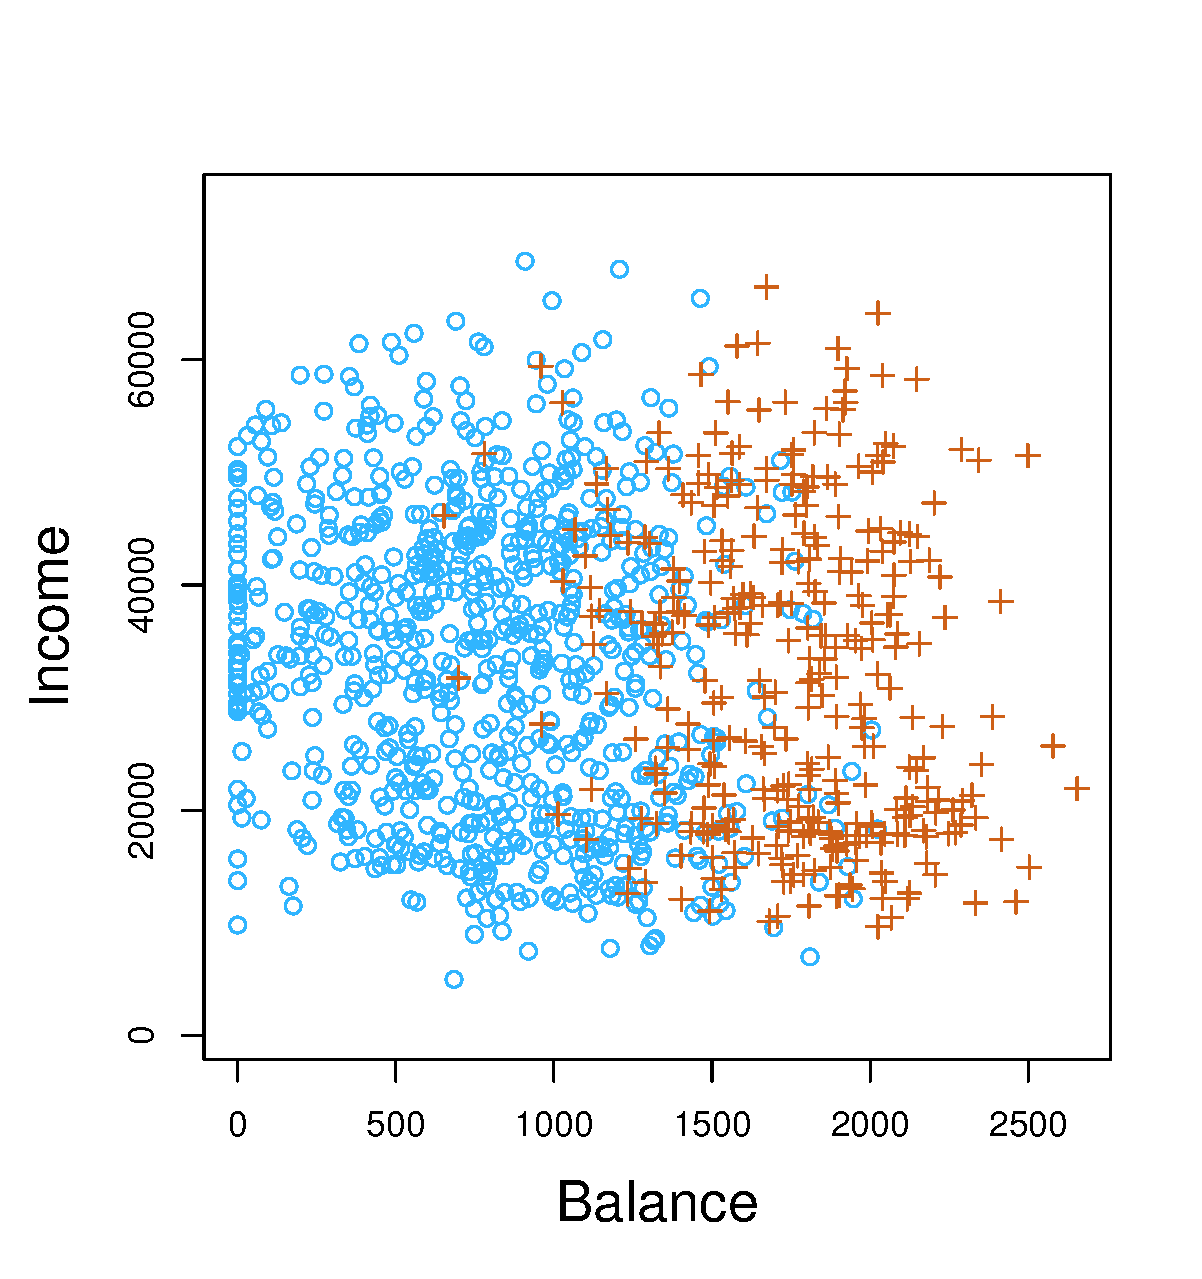
\includegraphics[width=\textwidth,height=0.65\textheight,keepaspectratio]{4_1a.pdf}
    \end{column}
  \end{columns}
  \islpsource{Figure 4.1}
\end{frame}

\begin{frame}{Why ordinary linear regression fails on 0/1 data}
  Tempting answer: code $Y = 1$ for default, $Y = 0$ otherwise, and
  run OLS. Three reasons this fails.
  \begin{alertblock}{Three problems}
    \begin{enumerate}
      \item Predictions can fall \emph{outside $[0, 1]$} --- nonsensical
            as probabilities.
      \item For $K > 2$ classes, the implicit numerical coding
            ($1, 2, 3$) imposes an arbitrary ordering and arbitrary
            distances.
      \item Errors are heteroscedastic by construction:
            $\mathrm{Var}(Y \mid X) = p(1-p)$ depends on $X$.
    \end{enumerate}
  \end{alertblock}
  We need a model that produces well-calibrated probabilities and
  handles multiple classes naturally.
\end{frame}


% ============================================================

% ---------------- Exercise 4.1 ----------------
\begin{frame}{Exercise 4.1 \textemdash{} Why not linear regression? [Concept]}
\begin{exercise}
A colleague wants to predict a patient's emergency diagnosis, coding the
three unordered categories as $Y=1$ (stroke), $Y=2$ (overdose),
$Y=3$ (seizure), and fitting ordinary least squares (OLS).
\begin{enumerate}
  \item What implicit assumption does the coding $1,2,3$ impose on the
        three diagnoses, and why is it inappropriate here?
  \item Suppose instead there are only two classes coded $0/1$ and we fit
        OLS. Name two problems with the fitted values as probabilities.
  \item Would relabelling the classes change the OLS fit? What does your
        answer imply about using linear regression here?
\end{enumerate}
\end{exercise}
\end{frame}

\begin{frame}{Solution \textemdash{} Exercise 4.1 (1/2)}
\begin{solutionbox}
\textbf{Method.} Ask what the numerical coding \emph{implicitly assumes}
about the response, then check each assumption against what a
probability model must deliver.

\vspace{1mm}
\textbf{(1) The coding imposes order and equal spacing.}
Using $1,2,3$ tells the model that stroke $<$ overdose $<$ seizure and
that the ``distance'' from stroke to overdose equals that from overdose
to seizure. The diagnoses are \emph{unordered categories}; any such
ordering and spacing is arbitrary and has no medical meaning.
Concretely, a fitted value of $1.5$ would assert a patient is
``halfway between stroke and overdose'' --- clinically meaningless.

\vspace{1mm}
\textbf{(2) Two problems with OLS on a $0/1$ response.}
\begin{itemize}
  \item Fitted values are unbounded, so predictions can fall
        \emph{outside} $[0,1]$ and cannot be read as probabilities
        (e.g.\ a \emph{negative} ``default probability'').
  \item The errors are heteroscedastic by construction:
        $\mathrm{Var}(Y\mid X)=p(1-p)$ depends on $X$, violating the
        constant-variance assumption of OLS --- so its standard errors
        and $p$-values are invalid as well.
\end{itemize}
\end{solutionbox}
\end{frame}

\begin{frame}{Solution \textemdash{} Exercise 4.1 (2/2)}
\begin{solutionbox}
\textbf{(3) Yes, relabelling changes the fit.}
A different assignment of the numbers $1,2,3$ to the categories produces
a different response vector and hence a different least-squares model
and different predictions --- swapping the codes of stroke and seizure
reverses the fitted ordering although the data are unchanged. Because
the answer depends on an arbitrary
choice, linear regression is \emph{not appropriate} for an unordered
multiclass response. (For two classes, $0/1$ OLS happens to give the
same classification as LDA, but its fitted values are still not valid
probabilities.)

\vspace{1mm}
\textbf{Interpretation.} What we actually need is a model that outputs
calibrated probabilities in $(0,1)$ and treats the classes
symmetrically --- exactly the gap that logistic regression (two
classes) and its multinomial/softmax extension ($K>2$) fill in this
chapter.

\vspace{1mm}
\emph{Common mistake: hoping a larger sample fixes the problem. No
amount of data repairs an arbitrary coding --- the flaw sits in the
model specification, not in sampling noise.}
\end{solutionbox}
\end{frame}

\section{Logistic regression}
% ============================================================
\subsection{Building the model}

\begin{frame}{Why we need a logistic curve}
  We need to map any linear predictor $z = \beta_0 + \beta^\top x$ to a
  probability in $(0, 1)$.
  \vspace{-1mm}
  \begin{center}
    
\includegraphics[width=0.92\textwidth,height=0.40\textheight,keepaspectratio]{ch04_x_sigmoid.png}
  \end{center}
  \vspace{-2mm}
  \begin{takeaway}[The logistic function]
    $\sigma(z) = e^{z}/(1 + e^{z})$ is smooth, monotone $0\to1$, and
    symmetric about $\sigma(0) = 0.5$ (left). Its inverse, the
    \emph{logit}, stretches $(0,1)$ onto the whole real line (right) ---
    so a \emph{linear} model belongs on the logit scale.
  \end{takeaway}
\end{frame}

\begin{frame}{The logistic regression model}
  \begin{block}{Formal model}
    \[
      \boxed{\;
        p(X) := \Pr(Y = 1 \mid X)
        = \frac{e^{\beta_0 + \beta^\top X}}
               {1 + e^{\beta_0 + \beta^\top X}}.
      \;}
    \]
  \end{block}
  Equivalently, the \emph{log-odds} (logit) are linear:
  \[
    \log\!\left(\frac{p(X)}{1 - p(X)}\right)
     = \beta_0 + \beta_1 X_1 + \cdots + \beta_p X_p.
  \]
  \begin{takeaway}[Why two forms?]
    They are the \emph{same} model written two ways. The first guarantees
    $p(X) \in (0,1)$; the second shows the model is linear on the
    log-odds scale --- so all the intuition from Chapter 3 carries over,
    just on a transformed response.
  \end{takeaway}
\end{frame}

\begin{frame}{Reading the model symbol-by-symbol}
  \begin{readme}
    \begin{tabular}{@{}cl@{}}
      \toprule
      \textbf{Symbol} & \textbf{Meaning} \\
      \midrule
      $Y$         & Binary response, $0$ or $1$ \\
      $p(X)$      & $\Pr(Y = 1 \mid X)$, the conditional probability \\
      $p(X) / (1 - p(X))$ & The \emph{odds} of $Y = 1$ \\
      $\log[p / (1-p)]$ & The \emph{log-odds} or logit, in $(-\infty, +\infty)$ \\
      $\beta_j$   & Effect of $X_j$ on the \emph{log-odds} \\
      $e^{\beta_j}$ & Multiplicative effect of $X_j$ on the \emph{odds} \\
      \bottomrule
    \end{tabular}
  \end{readme}
  \begin{takeaway}[Why the logit?]
    The log-odds are unbounded, so a linear model on this scale is
    natural. The sigmoid then squashes back into $(0, 1)$.
  \end{takeaway}
\end{frame}

\begin{frame}{The logistic curve in pictures}
  \begin{center}
    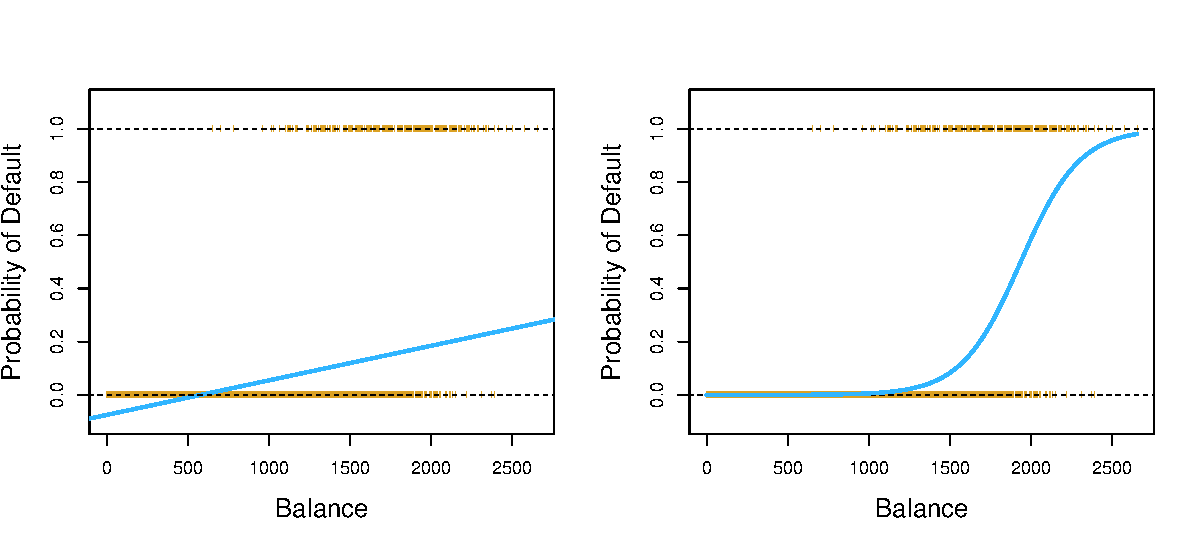
\includegraphics[width=0.78\textwidth,height=0.62\textheight,keepaspectratio]{4_2.pdf}
  \end{center}
  Linear regression (left) versus logistic regression (right).
  Logistic regression keeps probabilities in $[0, 1]$ everywhere.
  \islpsource{Figure 4.2}
\end{frame}

\begin{frame}{Recreating Figure 4.2 on the Default data}
  \begin{center}
    
\includegraphics[width=0.95\textwidth,height=0.6\textheight,keepaspectratio]{ch04_logistic_vs_linear.png}
  \end{center}
  \begin{takeaway}
    Fitting a straight line to the $0/1$ default indicator (left) drives
    predicted probabilities \emph{below zero} at small balances. The
    logistic curve (right) stays inside $[0,1]$ by construction.
  \end{takeaway}
\end{frame}


% ---------------- Exercise 4.2 ----------------
\begin{frame}{Exercise 4.2 \textemdash{} Computing $p(X)$ from coefficients [Math]}
\begin{exercise}
A simple logistic regression of \texttt{default} on \texttt{balance}
gives log-odds $\eta = \beta_0 + \beta_1\,\text{balance}$ with
$\hat\beta_0 = -10.65$ and $\hat\beta_1 = 0.0055$ (per dollar).
For a customer with a balance of \$1{,}500:
\begin{enumerate}
  \item Compute the log-odds $\eta$.
  \item Compute the probability of default $p(X)$.
  \item Compute the odds of default and relate them to part (1).
  \item At what balance does the model give $p(X)=0.5$?
\end{enumerate}
\end{exercise}
\end{frame}

\begin{frame}{Solution \textemdash{} Exercise 4.2 (1/2)}
\begin{solutionbox}
\textbf{Method.} Everything follows one pipeline:
balance $\xrightarrow{\text{linear}}$ log-odds $\eta$
$\xrightarrow{\exp}$ odds $e^{\eta}$
$\xrightarrow{\text{normalise}}$ probability
$p=e^{\eta}/(1+e^{\eta})$.

\vspace{1mm}
\textbf{(1) Log-odds.} Substitute the balance into the linear predictor:
\[
  \eta = -10.65 + 0.0055 \times 1500 = -10.65 + 8.25 = -2.40 .
\]
Negative log-odds already signal $p<0.5$; the customer looks safe.

\vspace{1mm}
\textbf{(2) Probability.} Push $\eta$ through the sigmoid
(needed because $\eta$ itself lives on $(-\infty,\infty)$, not $[0,1]$):
\[
  p = \frac{e^{\eta}}{1+e^{\eta}} = \frac{e^{-2.40}}{1+e^{-2.40}}
    = \frac{0.0907}{1.0907} \approx 0.083 \;(8.3\%).
\]
\end{solutionbox}
\end{frame}

\begin{frame}{Solution \textemdash{} Exercise 4.2 (2/2)}
\begin{solutionbox}
\textbf{(3) Odds.}
\[
  \text{odds} = \frac{p}{1-p} = e^{\eta} = e^{-2.40} \approx 0.091
  \qquad\Bigl(\text{check: } \tfrac{0.083}{0.917}\approx 0.091\ \checkmark\Bigr).
\]
The odds are exactly $\exp(\text{log-odds})$ from part (1): about one
default for every eleven non-defaults at this balance.

\vspace{1mm}
\textbf{(4) Balance giving $p=0.5$.}
$p=0.5 \iff \text{odds}=1 \iff \eta=0$ (since $\sigma(0)=\tfrac12$), so
solve the linear equation
\[
  0 = -10.65 + 0.0055\,\text{balance}
  \;\Longrightarrow\;
  \text{balance} = \frac{10.65}{0.0055} \approx 1936.4 \approx \$1{,}936 .
\]

\textbf{Interpretation.} Under a $0.5$ threshold the model flags
customers above $\approx\$1{,}936$; at \$1{,}500 our customer sits
clearly on the safe side with $p\approx 8\%$.

\vspace{1mm}
\emph{Common mistake: reading $\eta=-2.40$ itself as a probability.
Log-odds must first be pushed through the sigmoid --- probabilities can
never be negative.}
\end{solutionbox}
\end{frame}

\subsection{Estimating the coefficients}

\begin{frame}{Maximum likelihood: the recipe}
  Given data $(x_i, y_i)$ with $y_i \in \{0, 1\}$, build the
  likelihood:
  \begin{block}{Likelihood}
    \[
      L(\boldsymbol\beta) = \prod_{i: y_i = 1} p(x_i)
                            \prod_{i: y_i = 0} (1 - p(x_i)).
    \]
  \end{block}
  \begin{readme}
    Each customer who \emph{did} default contributes $p(x_i)$ to the
    product; each who \emph{did not} default contributes
    $1 - p(x_i)$. Taking logs turns the product into the sum we actually
    maximise (numerically --- there is no closed form):
    \[
      \log L(\boldsymbol\beta) = \sum_{i=1}^{n}
        \Big[\, y_i \log p(x_i) + (1 - y_i)\log\!\big(1 - p(x_i)\big)\,\Big].
    \]
  \end{readme}
\end{frame}

\begin{frame}{Three equivalent ways to think about the optimisation}
  \begin{itemize}
    \item \textbf{Maximum likelihood}: find $\hat\beta$ that makes the
          observed data most probable under the model.
    \item \textbf{Cross-entropy minimisation}: $-\log L$ is exactly the
          binary cross-entropy loss --- the same objective deep nets use.
    \item \textbf{Iteratively reweighted least squares (IRLS)}: solve a
          sequence of weighted regressions. Equivalent to Newton's
          method on the log-likelihood.
  \end{itemize}
  \begin{takeaway}
    All three give the same $\hat\beta$. Which view to take is a matter
    of taste; deep-learning courses prefer cross-entropy, statistics
    courses prefer maximum likelihood.
  \end{takeaway}
\end{frame}

\begin{frame}{Interpreting the coefficients}
  \begin{block}{Three different interpretation scales}
    \begin{itemize}
      \item \textbf{Sign of $\beta_j$}: increasing $X_j$ raises (positive)
            or lowers (negative) the probability of $Y = 1$.
      \item \textbf{$\exp(\beta_j)$}: multiplicative effect on the
            \emph{odds} of $Y = 1$.
      \item \textbf{Effect on probability}: nonlinear --- moves
            probabilities most in the middle of the curve, less at the
            extremes.
    \end{itemize}
  \end{block}
  \begin{takeaway}
    For interpretation, report $\exp(\beta_j)$, the \emph{odds ratio}: a
    single number with a clean ``holding the others fixed'' meaning. The
    probability effect has no such fixed value --- it depends on where you
    sit on the sigmoid.
  \end{takeaway}
\end{frame}

\begin{frame}{Worked example: Default vs.\ balance}
  Estimated $\hat\beta_{\text{balance}} \approx 0.0055$ in the Default
  data.
  \begin{numexample}[Three different scales]
    \textbf{Log-odds:} a \$1{,}000 increase in balance increases the
    log-odds of default by $0.0055 \cdot 1000 = 5.5$.\\[3pt]
    \textbf{Odds:} the odds multiply by $e^{5.5} \approx 245$.\\[3pt]
    \textbf{Probabilities:} at a balance of \$1{,}500 the model
    assigns about $8\,\%$ probability of default; at \$2{,}500 it
    assigns about $96\,\%$. Going up just \$1{,}000 lifts the
    probability from under $10\,\%$ to over $95\,\%$ because we are
    crossing the steep middle of the sigmoid.
  \end{numexample}
\end{frame}


% ---------------- Exercise 4.3 ----------------
\begin{frame}{Exercise 4.3 \textemdash{} Coefficients on the odds scale [Math]}
\begin{exercise}
A \emph{multiple} logistic regression on the Default data gives
$\hat\beta_0=-10.87$, $\hat\beta_{\text{balance}}=0.00574$,
$\hat\beta_{\text{income}}=0.003$ (per \$1{,}000), and
$\hat\beta_{\text{student[Yes]}}=-0.6468$.
\begin{enumerate}
  \item Interpret $e^{\hat\beta_{\text{student}}}$. By what percentage
        do the odds of default differ for a student versus a non-student
        at the \emph{same} balance and income?
  \item By what factor do the odds of default change for a \$200 increase
        in balance, holding the other predictors fixed?
  \item Why do we report a \emph{constant} multiplicative effect on the
        odds, but not on the probability?
\end{enumerate}
\end{exercise}
\end{frame}

\begin{frame}{Solution \textemdash{} Exercise 4.3 (1/2)}
\begin{solutionbox}
\textbf{Method.} Because the logit is linear, any coefficient converts
to an odds statement through one operation:
$\text{odds ratio} = e^{\beta_j\,\Delta X_j}$, ``holding the other
predictors fixed''.

\vspace{1mm}
\textbf{(1) Student effect.}
\[
  e^{\hat\beta_{\text{student}}} = e^{-0.6468} \approx 0.524 .
\]
Holding balance and income fixed, being a student multiplies the odds
of default by $0.524$ --- i.e.\ a student's odds are about
$1-0.524 = 47.6\%$ \emph{lower} than an otherwise identical
non-student. (This is the \emph{adjusted} effect; the unadjusted
comparison points the other way --- the student paradox.)

\vspace{1mm}
\textbf{(2) A \$200 increase in balance.} The log-odds shift by
$\Delta\eta = 0.00574 \times 200 = 1.148$, so the odds multiply by
\[
  e^{\,0.00574 \times 200} = e^{1.148} \approx 3.15 ,
\]
and this factor is the same whether balance goes
$500\to700$ or $1{,}500\to1{,}700$.
\end{solutionbox}
\end{frame}

\begin{frame}{Solution \textemdash{} Exercise 4.3 (2/2)}
\begin{solutionbox}
\textbf{(3) Odds vs.\ probability.}
Because the logit is \emph{linear}, a fixed change $\Delta X_j$ shifts
the log-odds by the constant $\beta_j\,\Delta X_j$, so the odds scale by
the constant factor $e^{\beta_j \Delta X_j}$ regardless of the starting
point. The probability, however, is the nonlinear sigmoid of the
log-odds, so no constant probability effect exists.

\vspace{1mm}
\textbf{Seeing it with numbers} (odds ratio $3.15$ from part 2):
\[
\begin{aligned}
  p=0.10:&\ \text{odds } \tfrac{0.10}{0.90}=0.111
    \xrightarrow{\times 3.15} 0.350
    \Rightarrow p=\tfrac{0.350}{1.350}\approx 0.26\ (+16\ \text{pts}),\\
  p=0.90:&\ \text{odds } \tfrac{0.90}{0.10}=9
    \xrightarrow{\times 3.15} 28.4
    \Rightarrow p=\tfrac{28.4}{29.4}\approx 0.97\ (+7\ \text{pts}).
\end{aligned}
\]
Same odds ratio, very different probability moves --- which is why the
odds scale is the one with a clean single-number interpretation.

\vspace{1mm}
\emph{Common mistake: reporting part (1) as ``students are $47.6\%$
less likely to default''. The reduction is in the \emph{odds}, not the
probability; the two only coincide approximately when the event is
rare.}
\end{solutionbox}
\end{frame}

\subsection{Multiple predictors and confounding}

\begin{frame}{Multiple logistic regression: the model}
  \begin{block}{Formal model}
    \[
      \log\frac{p(X)}{1 - p(X)}
        = \beta_0 + \beta_1 X_1 + \cdots + \beta_p X_p.
    \]
  \end{block}
  Same machinery as the simple case --- and the same warnings as in
  Chapter 3:
  \begin{itemize}
    \item Univariate slopes can mislead under confounding.
    \item ``Holding others fixed'' interpretation applies to each
          coefficient.
    \item Confounders can flip the sign of an estimated effect.
  \end{itemize}
  \begin{takeaway}
    Each $\beta_j$ is now an \emph{adjusted} effect --- the impact of
    $X_j$ with the other predictors held fixed. That adjustment is what
    lets the model untangle the confounding on the next slide.
  \end{takeaway}
\end{frame}

\begin{frame}{The student paradox in the Default data}
  \begin{alertblock}{What looks one way alone, another way together}
    In a univariate logistic regression, \texttt{student} appears
    \emph{more} default-prone than non-students. But controlling for
    \texttt{balance}, students are in fact \emph{less} likely to
    default at the same balance --- they simply tend to carry larger
    balances overall.
  \end{alertblock}
  \begin{takeaway}
    A textbook case of confounding. Always run multiple logistic
    regression when several predictors might be related.
  \end{takeaway}
\end{frame}

\begin{frame}{The student paradox visualised}
  \begin{center}
    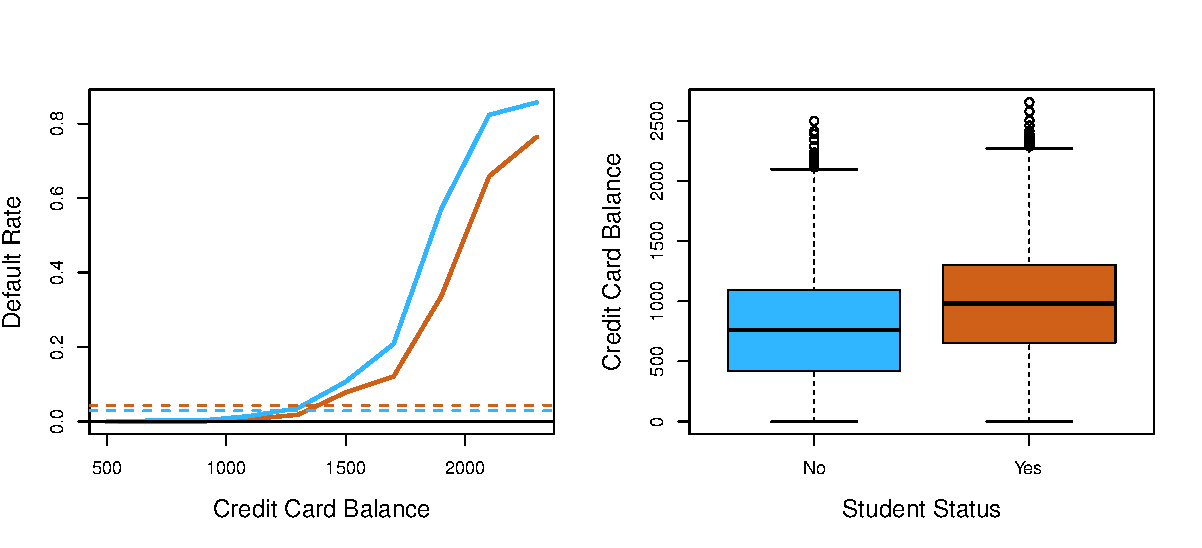
\includegraphics[width=0.85\textwidth,height=0.66\textheight,keepaspectratio]{4_3.pdf}
  \end{center}
  Conditional on balance, the orange (student) curve sits below the
  blue (non-student) curve. The univariate marginal told the opposite
  story.
  \islpsource{Figure 4.3}
\end{frame}


% ---------------- Exercise 4.4 ----------------
\begin{frame}{Exercise 4.4 \textemdash{} From probability to decision [Math]}
\begin{exercise}
Use the simple model $\eta = -10.65 + 0.0055\,\text{balance}$.
Three applicants have balances \$1{,}800, \$2{,}000 and \$2{,}200.
\begin{enumerate}
  \item Compute the predicted probability of default for each.
  \item Using the default threshold $0.5$ (predict ``default'' if
        $p>0.5$), classify each applicant.
  \item The bank now lowers the threshold to $0.2$ to catch more
        defaulters. What is the new decision boundary (in dollars of
        balance), and which classifications change?
\end{enumerate}
\end{exercise}
\end{frame}

\begin{frame}{Solution \textemdash{} Exercise 4.4 (1/2)}
\begin{solutionbox}
\textbf{Method.} For each applicant compute
$\eta=-10.65+0.0055\times\text{balance}$, then
$p=e^{\eta}/(1+e^{\eta})$; a threshold on $p$ is equivalent to a
threshold on $\eta$, i.e.\ to a dollar boundary on balance.

\vspace{1mm}
\textbf{(1) Probabilities} (substituting each balance):
\[
\begin{aligned}
  \$1{,}800:&\ \eta=-10.65+9.90=-0.75,\ p=\tfrac{e^{-0.75}}{1+e^{-0.75}}
              =\tfrac{0.472}{1.472}\approx 0.321,\\
  \$2{,}000:&\ \eta=-10.65+11.00=0.35,\ p=\tfrac{e^{0.35}}{1+e^{0.35}}
              =\tfrac{1.419}{2.419}\approx 0.587,\\
  \$2{,}200:&\ \eta=-10.65+12.10=1.45,\ p=\tfrac{e^{1.45}}{1+e^{1.45}}
              =\tfrac{4.263}{5.263}\approx 0.810.
\end{aligned}
\]
Note the balances are evenly spaced (\$200 apart) but the probability
steps are not ($+0.27$, then $+0.22$) --- the sigmoid is nonlinear.
\end{solutionbox}
\end{frame}

\begin{frame}{Solution \textemdash{} Exercise 4.4 (2/2)}
\begin{solutionbox}
\textbf{(2) Threshold $0.5$.}
$p>0.5 \iff \eta>0 \iff \text{balance} > \tfrac{10.65}{0.0055}
\approx \$1{,}936$. So
\$1{,}800 $\to$ \textbf{No}, \$2{,}000 $\to$ \textbf{Yes},
\$2{,}200 $\to$ \textbf{Yes} --- consistent with the probabilities
$0.321 < 0.5 < 0.587 < 0.810$ from part (1).

\vspace{1mm}
\textbf{(3) Threshold $0.2$.}
First convert the probability threshold to the log-odds scale:
$p=0.2 \iff \eta=\log\!\frac{0.2}{0.8}=\log 0.25 = -1.386$. Then solve
for the dollar boundary:
\[
  \text{balance} = \frac{-1.386 + 10.65}{0.0055}
                 = \frac{9.264}{0.0055} \approx \$1{,}684 .
\]
Every applicant above \$1{,}684 is flagged: the \$1{,}800 applicant
flips from \textbf{No} to \textbf{Yes}; the other two remain
\textbf{Yes}.

\vspace{1mm}
\textbf{Interpretation.} Lowering the threshold slides the dollar
boundary left ($1{,}936\to1{,}684$): sensitivity rises (more true
defaulters caught) at the price of more false positives. The right
cutoff depends on the bank's cost ratio of the two errors.

\vspace{1mm}
\emph{Common mistake: applying the new threshold on the wrong scale ---
requiring $\eta>0.2$ instead of $\eta>\log(0.2/0.8)=-1.386$.}
\end{solutionbox}
\end{frame}

\subsection{Multinomial extension}

\begin{frame}{From two classes to $K$: the softmax}
  \begin{block}{Multinomial logistic model}
    Pick a baseline class (say $K$) and set:
    \[
      \Pr(Y = k \mid X)
      = \frac{e^{\beta_{k0} + \beta_{k}^\top X}}
             {1 + \sum_{\ell=1}^{K-1} e^{\beta_{\ell 0} + \beta_\ell^\top X}}.
    \]
  \end{block}
  \begin{readme}
    Coefficients depend on the chosen baseline, but predictions are
    invariant to the choice. The equivalent symmetric ``softmax''
    parameterisation removes the need for a baseline --- this is the
    form used in deep learning.
  \end{readme}
  \begin{takeaway}
    The $K$ outputs are non-negative and sum to $1$ by construction, so
    they are genuine probabilities. Predict the class with the largest
    numerator.
  \end{takeaway}
\end{frame}


\begin{frame}{Mini-check: interpreting logistic coefficients}
  \begin{readme}[Self-assessment]
    A logistic regression on customer-default data gives
    $\hat\beta_{\text{balance}} = 0.0055$ (per dollar of balance).
    \begin{enumerate}
      \item By how much does the \emph{log-odds} change for a \$500
            increase in balance?
      \item By how much do the \emph{odds} change for a \$500 increase?
      \item Why is the change in \emph{probability} not
            proportional to $\beta$?
    \end{enumerate}
  \end{readme}
  \begin{takeaway}[Answers]
    1.\ $0.0055 \cdot 500 = 2.75$ on the log-odds scale.\quad
    2.\ Multiplied by $e^{2.75} \approx 15.6$.\quad
    3.\ The sigmoid is nonlinear --- the same $\Delta\beta$ moves the
        probability differently depending on where on the curve you are.
  \end{takeaway}
\end{frame}

% ---------------- Extended Exercise 4.1 ----------------
\begin{frame}{Extended Exercise 4.1 \textemdash{} Logistic regression end-to-end [Math]}
\begin{longexercise}
A multiple logistic regression on the Default data estimates the log-odds
of default as
$\eta=\beta_0+\beta_1\,\text{balance}+\beta_2\,\text{income}
      +\beta_3\,\text{student}$, with
$\beta_0=-10.869$, $\beta_1=0.00574$ (per \$1 of balance),
$\beta_2=0.003$ (per \$1{,}000 of income) and
$\beta_3=-0.6468$ (student${}={}$Yes). Two customers:
\emph{A} --- non-student, balance \$1{,}000, income \$40{,}000;\quad
\emph{B} --- student, balance \$2{,}000, income \$30{,}000.
\begin{enumerate}
  \item Compute the log-odds $\eta$ and probability $p(X)$ for A and B.
  \item For A, compute the odds of default and relate them to $\eta$.
  \item By what factor do the odds change for a \$100 increase in balance
        (others fixed)? Interpret $e^{\beta}$.
  \item Interpret $e^{\beta_3}$: how do a student's odds compare with an
        identical non-student's?
  \item Find the balance at which $p=0.5$ for a non-student with
        \$40{,}000 income (the decision boundary); note how it shifts for
        a student.
  \item In one sentence, how are the $\beta$'s estimated?
\end{enumerate}
\end{longexercise}
\end{frame}

\begin{frame}{Solution \textemdash{} Extended Exercise 4.1 (1/3)}
\begin{solutionbox}
\textbf{Method.} Assemble $\eta$ term by term --- watching units:
income enters in \$1{,}000s --- then map to a probability with the
sigmoid.

\vspace{1mm}
\textbf{(1) Log-odds and probabilities:}
\[
\begin{aligned}
  \eta_A&=-10.869+0.00574(1000)+0.003(40)
         =-10.869+5.740+0.120=-5.009,\\
  \eta_B&=-10.869+0.00574(2000)+0.003(30)-0.6468\\
        &=-10.869+11.480+0.090-0.647=0.054.
\end{aligned}
\]
Then $p=\sigma(\eta)=e^{\eta}/(1+e^{\eta})$ gives
$p_A=\tfrac{e^{-5.009}}{1+e^{-5.009}}=\tfrac{0.0067}{1.0067}
\approx 0.0066\ (0.66\%)$ and
$p_B=\tfrac{e^{0.054}}{1+e^{0.054}}=\tfrac{1.055}{2.055}
\approx 0.514\ (51.4\%)$: A is a very safe customer; B sits right at
the knife edge.
\end{solutionbox}
\end{frame}

\begin{frame}{Solution \textemdash{} Extended Exercise 4.1 (2/3)}
\begin{solutionbox}
\textbf{(2) Odds for A.}
$\text{odds}_A=\dfrac{p_A}{1-p_A}=e^{\eta_A}=e^{-5.009}\approx 0.0067$ ---
about one default per $150$ non-defaults. The odds are exactly
$\exp(\text{log-odds})$.

\vspace{1mm}
\textbf{(3) A \$100 increase in balance.}
$\Delta\eta=\beta_1\cdot 100=0.574$, so the odds multiply by
$e^{0.574}\approx 1.78$: every extra \$100 of balance raises the odds of
default by about $78\%$, \emph{regardless} of the starting point
(constant on the odds scale because the logit is linear).

\vspace{1mm}
\textbf{(4) Student effect.}
$e^{\beta_3}=e^{-0.6468}\approx 0.524$. Holding balance and income fixed,
a student's odds of default are $0.524\times$ those of an identical
non-student --- about $47.6\%$ lower.
\end{solutionbox}
\end{frame}

\begin{frame}{Solution \textemdash{} Extended Exercise 4.1 (3/3)}
\begin{solutionbox}
\textbf{(5) Decision boundary} ($p=0.5\iff\eta=0$). For a non-student with
\$40{,}000 income,
\[
  0=-10.869+0.00574\,\text{balance}+0.12
  \;\Rightarrow\;
  \text{balance}^\star=\frac{10.869-0.12}{0.00574}\approx \$1{,}873 .
\]
Above $\approx\$1{,}873$ the model predicts default at a $0.5$ cutoff. For
a \emph{student} the boundary rises to
$\frac{10.869-0.12+0.6468}{0.00574}\approx \$1{,}985$: a student needs a
larger balance to reach the same $50\%$ risk --- the same message as (4).

\vspace{1mm}
\textbf{(6) Estimation.}
By \emph{maximum likelihood}: choose $\beta$ to maximise
$L(\beta)=\prod_{y_i=1}p(x_i)\prod_{y_i=0}\bigl(1-p(x_i)\bigr)$
(equivalently minimise the cross-entropy $-\log L$). There is no closed
form, so software solves it numerically (Newton / IRLS) --- conceptually,
pick the coefficients that make the observed Yes/No pattern most probable.

\vspace{1mm}
\emph{Common mistake: plugging income in dollars. $\beta_2=0.003$ is
per \$1{,}000, so use $0.003\times 40$, not $0.003\times 40{,}000$ ---
the latter adds $120$ to $\eta$ and drives every probability to $1$.}
\end{solutionbox}
\end{frame}

% ============================================================
\section{Generative models}
% ============================================================
\subsection{Bayes refresher}

\begin{frame}{Two philosophies of classification}
  \begin{columns}[T]
    \begin{column}{0.48\textwidth}
      \begin{block}{Discriminative}
        Model $\Pr(Y \mid X)$ directly. \emph{Logistic regression}
        does this.
      \end{block}
    \end{column}
    \begin{column}{0.48\textwidth}
      \begin{block}{Generative}
        Model the priors $\pi_k$ and class-conditional densities
        $f_k(X)$, then apply Bayes' rule.
      \end{block}
    \end{column}
  \end{columns}
  \begin{takeaway}[Which to prefer?]
    Discriminative models assume \emph{less} and often predict better
    when data are plentiful. Generative models (LDA, QDA, naive Bayes)
    add structure through $f_k$, which pays off when $n$ is small, when
    classes are well separated, or when some features are missing ---
    situations where logistic regression can be unstable.
  \end{takeaway}
\end{frame}

\begin{frame}{Bayes' theorem in the classification setting}
  \begin{block}{Bayes posterior}
    \[
      \boxed{\;
        \Pr(Y = k \mid X = x)
          = \frac{\pi_k\, f_k(x)}{\sum_{\ell=1}^K \pi_\ell\, f_\ell(x)}.
      \;}
    \]
  \end{block}
  Read it as \textbf{posterior} $\propto$ \textbf{prior} $\times$
  \textbf{likelihood}: the numerator scores class $k$, and the
  denominator merely renormalises so the $K$ posteriors sum to one.
  \begin{readme}
    \begin{tabular}{@{}cl@{}}
      \toprule
      \textbf{Symbol} & \textbf{Meaning} \\
      \midrule
      $\pi_k = \Pr(Y = k)$ & Prior class probability (easy: class
                              proportions in the training data) \\
      $f_k(x)$ & Class-conditional density of $X$ given $Y = k$ \\
      \bottomrule
    \end{tabular}
  \end{readme}
  Generative methods differ in \emph{how} they estimate $f_k$.
\end{frame}

\begin{frame}{Bayes' theorem as a flow: prior $\times$ likelihood $\to$ posterior}
  \begin{center}
  \resizebox{\textwidth}{!}{%
  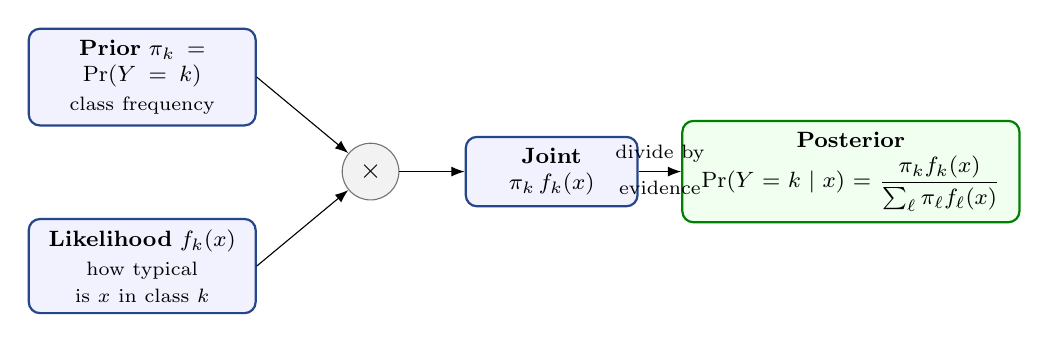
\begin{tikzpicture}[font=\footnotesize,>=Latex,
      box/.style={rounded corners,draw=accent,line width=0.8pt,fill=blue!5,
                  align=center,inner sep=4pt},
      op/.style={circle,draw=black!55,fill=black!5,minimum size=0.72cm,
                 inner sep=0pt,font=\normalsize}]
    \node[box,text width=2.6cm] (prior) at (0,1.2)
      {\textbf{Prior} $\pi_k=\Pr(Y=k)$\\[1pt]\scriptsize class frequency};
    \node[box,text width=2.6cm] (lik) at (0,-1.2)
      {\textbf{Likelihood} $f_k(x)$\\[1pt]\scriptsize how typical is $x$ in class $k$};
    \node[op] (times) at (2.9,0) {$\times$};
    \node[box,text width=1.9cm] (joint) at (5.2,0)
      {\textbf{Joint} $\pi_k\,f_k(x)$};
    \node[box,text width=4.0cm,fill=green!6,draw=green!50!black] (post) at (9.0,0)
      {\textbf{Posterior}\\[2pt]
       $\displaystyle\Pr(Y=k\mid x)=\frac{\pi_k f_k(x)}{\sum_\ell \pi_\ell f_\ell(x)}$};
    \draw[->] (prior.east) -- (times);
    \draw[->] (lik.east)   -- (times);
    \draw[->] (times) -- (joint);
    \draw[->] (joint) -- node[above=0pt,font=\scriptsize]{divide by}
                          node[below=0pt,font=\scriptsize]{evidence} (post);
  \end{tikzpicture}}
  \end{center}
  \begin{takeaway}
    Every generative classifier --- LDA, QDA, naive Bayes --- \emph{is}
    this same flow. They differ only in \emph{how they model the
    likelihood} $f_k(x)$. Classify $x$ to the class with the largest
    posterior.
  \end{takeaway}
\end{frame}

\subsection{LDA}

\begin{frame}{Linear Discriminant Analysis: the assumption}
  \begin{block}{Assumption}
    Within each class $k$, the predictor vector $X$ is multivariate
    normal with class-specific mean $\mu_k$ but a \emph{common}
    covariance matrix $\Sigma$.
  \end{block}
  \begin{takeaway}[Why this assumption is interesting]
    With a common $\Sigma$, the difference between two posterior
    log-probabilities reduces to a \emph{linear} function of $x$. So
    LDA gives linear decision boundaries --- by assumption, not by
    design.
  \end{takeaway}
\end{frame}

\begin{frame}{The LDA discriminant}
  Plugging Gaussian densities into Bayes' rule and dropping common
  factors leaves the linear discriminant:
  \begin{block}{LDA discriminant}
    \[
      \boxed{\;
        \delta_k(x) = x^\top \Sigma^{-1}\mu_k -
                     \tfrac12 \mu_k^\top \Sigma^{-1}\mu_k +
                     \log \pi_k.
      \;}
    \]
  \end{block}
  Classify $x$ to the class $k$ that maximises $\delta_k(x)$: it is a
  \emph{score}, not a probability --- larger means more evidence for
  class $k$. Because $\delta_k(x)$ is \emph{linear} in $x$, the boundary
  between any two classes is a straight line (hyperplane) --- the
  ``linear'' in LDA.
\end{frame}

\begin{frame}{Reading the LDA discriminant}
  \begin{readme}
    \begin{tabular}{@{}cl@{}}
      \toprule
      \textbf{Term} & \textbf{Role} \\
      \midrule
      $x^\top \Sigma^{-1}\mu_k$
        & Project $x$ onto the direction of class-$k$'s mean,
          weighted by $\Sigma^{-1}$ \\
      $-\tfrac12 \mu_k^\top \Sigma^{-1}\mu_k$
        & Penalty for distant means (a constant per class) \\
      $\log \pi_k$
        & Prior boost: bigger classes win ties \\
      \bottomrule
    \end{tabular}
  \end{readme}
  \begin{takeaway}
    LDA is a weighted nearest-mean classifier, with weights given by
    the (inverse) covariance and a prior tilt for class size.
  \end{takeaway}
\end{frame}

\begin{frame}{LDA decision boundary on simulated data}
  \begin{center}
    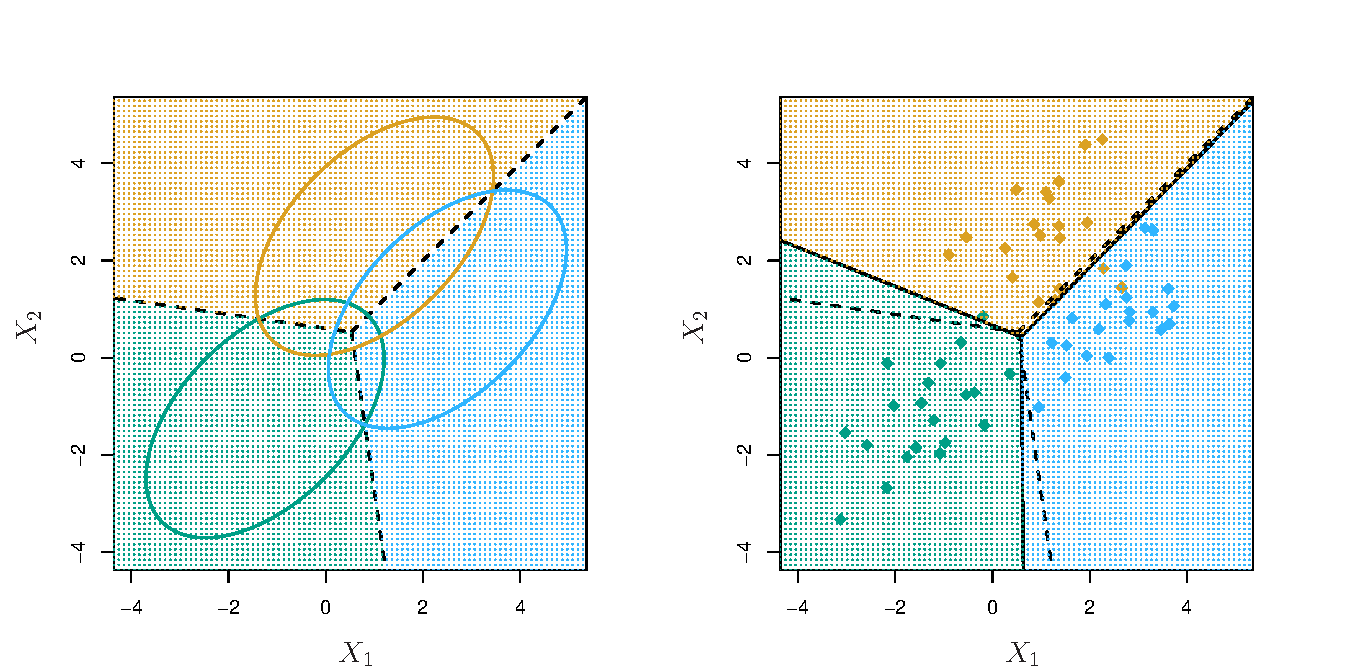
\includegraphics[width=0.85\textwidth,height=0.62\textheight,keepaspectratio]{4_6.pdf}
  \end{center}
  Two-class LDA on simulated Gaussians: dashed = Bayes optimum,
  solid = LDA estimated from training data. The two are very close.
  \islpsource{Figure 4.6}
\end{frame}

\begin{frame}{LDA with one predictor: two Gaussians and a cutoff}
  \begin{center}
\includegraphics[width=0.88\textwidth,height=0.5\textheight,keepaspectratio]{ch04_x_lda_1d_densities.png}\end{center}
  \begin{takeaway}LDA compares the prior-weighted densities $\pi_k f_k(x)$: equal priors put the cutoff at the midpoint $0$; $\pi_2 = 0.8$ slides it by $\ln(0.8/0.2)\,\sigma^2/(\mu_2{-}\mu_1) = 0.46$ toward the rarer class. The shaded overlap is error even Bayes cannot remove.\end{takeaway}
\end{frame}


% ---------------- Exercise 4.5 ----------------
\begin{frame}{Exercise 4.5 \textemdash{} LDA discriminant in one dimension [Math]}
\begin{exercise}
Two classes with $X\mid Y=k \sim \mathcal{N}(\mu_k,\sigma^2)$,
$\sigma^2=1$, $\mu_0=0$, $\mu_1=2$. Recall
$\delta_k(x)=x\dfrac{\mu_k}{\sigma^2}-\dfrac{\mu_k^2}{2\sigma^2}+\log\pi_k$.
\begin{enumerate}
  \item With equal priors, write $\delta_0,\delta_1$ and find the
        decision boundary.
  \item Classify $x=1.5$.
  \item Now take priors $\pi_0=0.8$, $\pi_1=0.2$. Recompute the boundary
        and reclassify $x=1.5$.
  \item Give the general boundary formula and check it against part (3).
\end{enumerate}
\end{exercise}
\end{frame}

\begin{frame}{Solution \textemdash{} Exercise 4.5 (1/2)}
\begin{solutionbox}
\textbf{Method.} With a shared variance we classify by the larger
discriminant score $\delta_k(x)$; the boundary is the $x$ where the two
scores tie. Substitute $\mu_0=0$, $\mu_1=2$, $\sigma^2=1$ throughout.

\vspace{1mm}
\textbf{(1) Equal priors.} Substituting into
$\delta_k(x)=x\mu_k/\sigma^2-\mu_k^2/(2\sigma^2)+\log\pi_k$:
\[
  \delta_0(x)=0+\log\tfrac12, \qquad
  \delta_1(x)=2x-\tfrac{4}{2}+\log\tfrac12 = 2x-2+\log\tfrac12 .
\]
The equal $\log\pi_k$ terms cancel in the comparison, leaving
$\delta_0=0$ vs.\ $\delta_1=2x-2$. Setting them equal:
$0=2x-2\Rightarrow x=1$ --- exactly the midpoint
$(\mu_0+\mu_1)/2$ of the means, as symmetry demands (equal priors,
equal spread). Assign class $1$ if $x>1$.

\vspace{1mm}
\textbf{(2)} $\delta_1(1.5)-\delta_0(1.5)=2(1.5)-2=1>0$, so
$x=1.5 \Rightarrow$ class $1$ (consistent with $1.5>1$).
\end{solutionbox}
\end{frame}

\begin{frame}{Solution \textemdash{} Exercise 4.5 (2/2)}
\begin{solutionbox}
\textbf{(3) Unequal priors.} Now the $\log\pi_k$ terms differ:
$\delta_0=\log 0.8=-0.223$ and $\delta_1=2x-2+\log 0.2=2x-2-1.609$.
Setting equal:
\[
  -0.223 = 2x - 3.609 \Rightarrow 2x = 3.386 \Rightarrow x = 1.693 .
\]
Assign class $1$ if $x>1.693$. Now $x=1.5<1.693 \Rightarrow$ class $0$:
same data point, opposite decision, purely because class $1$ became
rare --- the rarer class requires stronger evidence.

\vspace{1mm}
\textbf{(4) General boundary.}
\[
  x^\star = \frac{\mu_0+\mu_1}{2}
          - \frac{\sigma^2}{\mu_1-\mu_0}\log\frac{\pi_1}{\pi_0}.
\]
Check: $\dfrac{0+2}{2}-\dfrac{1}{2}\log\dfrac{0.2}{0.8}
= 1 - 0.5(-1.386) = 1.693.$ \checkmark\quad
The prior term shifts the midpoint by $+0.693$ \emph{toward the rare
class's mean}, enlarging the common class's region.

\vspace{1mm}
\emph{Common mistake: shifting the boundary toward the \emph{common}
class. Rarity penalises class $1$ through $\log\pi_1$, so the boundary
moves toward $\mu_1$ and class $0$ wins more of the axis.}
\end{solutionbox}
\end{frame}

\subsection{QDA}

\begin{frame}{Quadratic Discriminant Analysis: relaxing the assumption}
  \begin{block}{QDA assumption \& discriminant (quadratic in $x$)}
    Each class keeps its \emph{own} covariance,
    $X \mid Y = k \sim \mathcal{N}(\mu_k, \Sigma_k)$, giving
    \[
      \boxed{\;
      \delta_k(x) = -\tfrac12 (x - \mu_k)^\top \Sigma_k^{-1}(x - \mu_k)
         - \tfrac12 \log|\Sigma_k| + \log \pi_k. \;}
    \]
  \end{block}
  \begin{readme}
    \begin{tabular}{@{}cl@{}}
      \toprule
      \textbf{Term} & \textbf{Role} \\
      \midrule
      $-\tfrac12 (x-\mu_k)^\top \Sigma_k^{-1}(x-\mu_k)$
        & Squared (Mahalanobis) distance of $x$ from class-$k$'s centre \\
      $-\tfrac12 \log|\Sigma_k|$
        & Volume penalty: down-weights classes with large spread \\
      $\log \pi_k$ & Prior boost: bigger classes win ties \\
      \bottomrule
    \end{tabular}
  \end{readme}
  Since each $\Sigma_k$ differs, the $x^\top \Sigma_k^{-1} x$ term no
  longer cancels --- boundaries become \emph{ellipses or hyperbolas},
  not lines.
\end{frame}

\begin{frame}{LDA vs.\ QDA: a bias-variance choice}
  \begin{columns}[T]
    \begin{column}{0.48\textwidth}
      \begin{block}{LDA}
        Estimates one $\Sigma$ ($\sim p^2/2$ parameters).
        Lower variance; biased if class covariances really differ.
      \end{block}
    \end{column}
    \begin{column}{0.48\textwidth}
      \begin{block}{QDA}
        Estimates $K$ separate $\Sigma_k$ ($\sim K p^2/2$ parameters).
        Lower bias; high variance when $n$ is small.
      \end{block}
    \end{column}
  \end{columns}
  \begin{takeaway}[Practical rule]
    Use LDA when classes look similar in spread; use QDA when class
    covariances are visibly different and you have plenty of data per
    class.
  \end{takeaway}
\end{frame}

\begin{frame}{LDA vs.\ QDA: visual}
  \begin{center}
    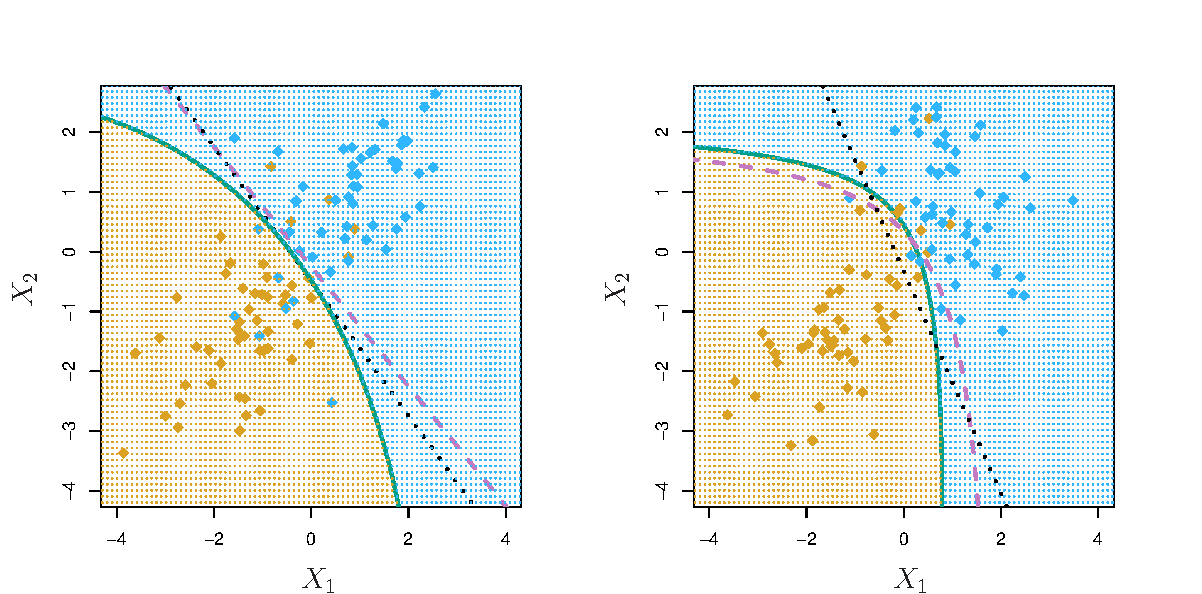
\includegraphics[width=0.92\textwidth,height=0.66\textheight,keepaspectratio]{4_9.pdf}
  \end{center}
  Equal covariances (left) $\Rightarrow$ LDA wins. Different
  covariances (right) $\Rightarrow$ QDA's curved boundary is closer
  to optimal.
  \islpsource{Figure 4.9}
\end{frame}

\begin{frame}{LDA vs.\ QDA decision boundaries (simulated)}
  \begin{center}
    
\includegraphics[width=0.95\textwidth,height=0.52\textheight,keepaspectratio]{ch04_lda_qda.png}
  \end{center}
  \begin{takeaway}
    Equal covariances (left): LDA's line all but coincides with QDA.
    Unequal covariances (right): only QDA's curved boundary tracks the
    true class structure.
  \end{takeaway}
\end{frame}


% ---------------- Exercise 4.6 ----------------
\begin{frame}{Exercise 4.6 \textemdash{} LDA vs.\ QDA: parameters and bias-variance [Concept]}
\begin{exercise}
Consider $K$ classes and $p$ predictors.
\begin{enumerate}
  \item How many free covariance parameters does LDA estimate?
        How many does QDA estimate?
  \item Evaluate both for $p=5$, $K=3$.
  \item Which method has higher variance, and which has higher bias?
        Under what condition is LDA's extra bias zero?
  \item State a practical rule for choosing between them.
\end{enumerate}
\end{exercise}
\end{frame}

\begin{frame}{Solution \textemdash{} Exercise 4.6 (1/2)}
\begin{solutionbox}
\textbf{Method.} Count the free entries in the covariance objects each
method must estimate; the difference is the extra variance QDA pays for
its extra flexibility.

\vspace{1mm}
\textbf{(1) Parameter counts.}
A covariance matrix is symmetric $p\times p$: $p$ variances on the
diagonal plus $p(p-1)/2$ distinct covariances off it, i.e.\
\[
  p + \frac{p(p-1)}{2} = \frac{p(p+1)}{2} \ \text{free entries.}
\]
LDA assumes one \emph{shared} $\Sigma$: $p(p+1)/2$ parameters.
QDA estimates one $\Sigma_k$ per class: $K\cdot p(p+1)/2$ parameters
--- the count scales with the number of classes.

\vspace{1mm}
\textbf{(2) For $p=5$, $K=3$.}
$p(p+1)/2 = 5\cdot 6/2 = 15$. LDA: $15$; QDA: $3\times 15 = 45$
covariance parameters. Both additionally estimate $Kp=15$ means and
$K-1=2$ free priors, so the totals are $15+15+2=32$ (LDA) vs.\
$45+15+2=62$ (QDA) --- QDA nearly doubles the parameter budget.
\end{solutionbox}
\end{frame}

\begin{frame}{Solution \textemdash{} Exercise 4.6 (2/2)}
\begin{solutionbox}
\textbf{(3) Bias-variance.}
QDA is more flexible: \emph{higher variance, lower bias} --- its extra
$30$ parameters (here) buy curved boundaries. LDA is more
rigid: \emph{lower variance, higher bias} --- but its extra bias is
\emph{zero when the true class covariances are actually equal}
($\Sigma_1=\dots=\Sigma_K$): then both methods target the same truth
and LDA gets there with fewer parameters, so it is preferable.

\vspace{1mm}
\textbf{(4) Rule of thumb.}
Use LDA when $n$ is small or the classes look similarly spread; use QDA
when the class covariances are visibly different and you have plenty of
data per class.

\vspace{1mm}
\textbf{Interpretation.} This is the Chapter~2 bias-variance trade-off
in classifier form: QDA is the ``more flexible'' model, and whether its
lower bias pays depends on how much data must stretch across
$K$ covariance matrices.

\vspace{1mm}
\emph{Common mistake: counting $p^2$ entries per covariance matrix ---
symmetry roughly halves the count to $p(p+1)/2$. And remember QDA's
count grows with $K$: many classes with few observations each is its
worst case.}
\end{solutionbox}
\end{frame}

\subsection{Naive Bayes}

\begin{frame}{Naive Bayes: extreme simplification}
  \begin{block}{The independence assumption}
    Within each class, the features are independent:
    $f_k(x) = \prod_{j=1}^p f_{kj}(x_j)$.
  \end{block}
  \begin{takeaway}
    The assumption is almost always wrong --- features are usually
    correlated. But the simplification massively reduces variance:
    each $f_{kj}$ is just a one-dimensional density.
  \end{takeaway}
  \begin{exampleblock}{Why it works in practice}
    Even when independence fails, naive Bayes often \emph{ranks}
    observations correctly --- which is all a classifier needs. It
    routinely beats more sophisticated methods when $n$ is small and
    $p$ is large.
  \end{exampleblock}
\end{frame}


% ============================================================

% ---------------- Exercise 4.7 ----------------
\begin{frame}{Exercise 4.7 \textemdash{} Naive Bayes from a small table [Math]}
\begin{exercise}
A spam filter has priors $\Pr(\text{Spam})=0.4$, $\Pr(\text{Ham})=0.6$
and two binary features: $F_1=$ ``contains the word \emph{free}'',
$F_2=$ ``contains a link''.
\begin{center}\small
\begin{tabular}{lcc}
\toprule
 & $\Pr(F_1=1\mid\cdot)$ & $\Pr(F_2=1\mid\cdot)$ \\
\midrule
Spam & 0.6 & 0.7 \\
Ham  & 0.1 & 0.2 \\
\bottomrule
\end{tabular}
\end{center}
A new email contains \emph{both} features.
\begin{enumerate}
  \item Using the conditional-independence assumption, compute the
        unnormalised score for each class.
  \item Compute $\Pr(\text{Spam}\mid F_1=1,F_2=1)$.
  \item Classify the email.
  \item What does the naive assumption buy you, and what does it cost?
\end{enumerate}
\end{exercise}
\end{frame}

\begin{frame}{Solution \textemdash{} Exercise 4.7 (1/2)}
\begin{solutionbox}
\textbf{Method.} Bayes' rule scores each class by its numerator
$\pi_k f_k(x)$; naive Bayes factorises the likelihood as
$f_k(x)=\prod_j\Pr(F_j\mid k)$. The denominator is common to both
classes, so we compare numerators first and normalise at the end.

\vspace{1mm}
\textbf{(1) Unnormalised scores} ($\pi_k\prod_j \Pr(F_j\mid k)$):
\[
\begin{aligned}
  \text{Spam}:&\ 0.4\times 0.6\times 0.7 = 0.4\times 0.42 = 0.168,\\
  \text{Ham}:&\ 0.6\times 0.1\times 0.2 = 0.6\times 0.02 = 0.012.
\end{aligned}
\]

\textbf{(2) Posterior.} Normalise by the sum $0.168+0.012=0.180$:
\[
  \Pr(\text{Spam}\mid F_1,F_2) = \frac{0.168}{0.180} \approx 0.933,
  \qquad
  \Pr(\text{Ham}\mid F_1,F_2) = \frac{0.012}{0.180} \approx 0.067 ,
\]
and the two posteriors sum to $1$. \checkmark
\end{solutionbox}
\end{frame}

\begin{frame}{Solution \textemdash{} Exercise 4.7 (2/2)}
\begin{solutionbox}
\textbf{(3) Decision.} $0.933>0.5 \Rightarrow$ classify as
\textbf{Spam}. In odds form: posterior odds
$=0.168/0.012 = 14$, the product of prior odds
$0.4/0.6=0.67$ and likelihood ratio $0.42/0.02=21$ --- the two features
overwhelm the prior that favoured Ham.

\vspace{1mm}
\textbf{(4) Trade-off.}
Assuming the features are independent \emph{within each class} means we
only estimate one-dimensional marginals $f_{kj}$ --- here just two
numbers per class instead of a joint table over all feature
combinations --- drastically reducing
the number of parameters and hence the variance. The cost is bias: the
assumption is usually false (e.g.\ e-mails containing \emph{free}
disproportionately also contain links), so the posterior
probabilities are miscalibrated --- yet the \emph{ranking} of
observations is often still good enough to classify well.

\vspace{1mm}
\emph{Common mistake: dropping the prior and normalising the
likelihoods alone --- $0.42/(0.42+0.02)\approx 0.955$ overstates the
spam probability. The prior matters; with rare positives it can flip
the decision outright.}
\end{solutionbox}
\end{frame}

% ---------------- Extended Exercise 4.2 ----------------
\begin{frame}{Extended Exercise 4.2 \textemdash{} LDA from Bayes' theorem [Math]}
\begin{longexercise}
Two classes with a single predictor $X$. Within class $k$,
$X\mid Y=k\sim\mathcal{N}(\mu_k,\sigma^2)$ with a \emph{shared} variance
$\sigma^2=4$ and means $\mu_0=1$, $\mu_1=5$. Priors $\pi_0=0.7$,
$\pi_1=0.3$.
\begin{enumerate}
  \item Starting from Bayes' theorem, show that comparing
        $\log[\pi_k f_k(x)]$ across classes reduces to the linear
        discriminant
        $\delta_k(x)=x\,\mu_k/\sigma^2-\mu_k^2/(2\sigma^2)+\log\pi_k$.
  \item Derive the decision boundary $x^\star$ where
        $\delta_0=\delta_1$; give the general formula and evaluate it.
  \item For $x=4$, compute $\delta_0,\delta_1$ and the posterior
        $\Pr(Y=1\mid x=4)$; classify the point.
  \item How does QDA change the derivation and the boundary?
\end{enumerate}
\end{longexercise}
\end{frame}

\begin{frame}{Solution \textemdash{} Extended Exercise 4.2 (1/3)}
\begin{solutionbox}
\textbf{Method.} Everything is Bayes' rule; the only algebra is
separating the terms that depend on $k$ from those that do not ---
possible precisely because $\sigma^2$ is shared.

\vspace{1mm}
\textbf{(1) Bayes $\Rightarrow$ linear discriminant.}
Bayes gives $\Pr(Y=k\mid x)=\pi_k f_k(x)/\sum_\ell \pi_\ell f_\ell(x)$;
the denominator is common, and $\log$ is monotone, so we classify by
the largest $\log[\pi_k f_k(x)]$. With
$f_k(x)=(2\pi\sigma^2)^{-1/2}e^{-(x-\mu_k)^2/(2\sigma^2)}$, expanding
the square $(x-\mu_k)^2 = x^2 - 2x\mu_k + \mu_k^2$ gives
\[
  \log[\pi_k f_k(x)]=
  \underbrace{-\tfrac12\log(2\pi\sigma^2)-\tfrac{x^2}{2\sigma^2}}_{\text{same for every class}}
  +\underbrace{x\tfrac{\mu_k}{\sigma^2}-\tfrac{\mu_k^2}{2\sigma^2}+\log\pi_k}_{=\;\delta_k(x)} .
\]
The first group is identical across classes ($\sigma^2$ shared, $x^2$ has
no $k$), so it cancels in any comparison, leaving the \emph{linear}
$\delta_k(x)$ --- this cancellation is the whole reason LDA's boundary
is a line.
\end{solutionbox}
\end{frame}

\begin{frame}{Solution \textemdash{} Extended Exercise 4.2 (2/3)}
\begin{solutionbox}
\textbf{(2) Boundary.} Set $\delta_0(x)=\delta_1(x)$ and solve;
substituting $\mu_0=1$, $\mu_1=5$, $\sigma^2=4$ and
$\log\frac{\pi_1}{\pi_0}=\log\frac{0.3}{0.7}=-0.847$:
\[
  x^\star=\frac{\mu_0+\mu_1}{2}
          -\frac{\sigma^2}{\mu_1-\mu_0}\log\frac{\pi_1}{\pi_0}
        =\frac{1+5}{2}-\frac{4}{4}(-0.847)
        =3+0.847=3.85 .
\]
Assign class $1$ if $x>3.85$. The prior tilt moves the boundary
$0.85$ units from the midpoint $3$ \emph{toward} the rarer class, which
needs stronger evidence.

\vspace{1mm}
\textbf{(3) Posterior at $x=4$.} Substituting into $\delta_k$:
\[
\begin{aligned}
  \delta_0(4)&=\tfrac{4\cdot1}{4}-\tfrac{1}{8}+\log 0.7
              =1-0.125-0.357=0.518,\\
  \delta_1(4)&=\tfrac{4\cdot5}{4}-\tfrac{25}{8}+\log 0.3
              =5-3.125-1.204=0.671.
\end{aligned}
\]
Since the dropped term cancels, the posterior is the softmax of the
$\delta_k$:
\[
  \Pr(Y=1\mid 4)=\frac{e^{0.671}}{e^{0.518}+e^{0.671}}
  =\frac{1.956}{1.679+1.956}\approx 0.538
  \;>0.5\Rightarrow\ \text{class } 1 ,
\]
consistent with $4>3.85$ --- but only barely: $x=4$ sits close to the
boundary, so the posterior is near $0.5$.
\end{solutionbox}
\end{frame}

\begin{frame}{Solution \textemdash{} Extended Exercise 4.2 (3/3)}
\begin{solutionbox}
\textbf{Cross-check via the raw densities.} With $\sigma=2$,
$f_k(4)=(2\pi\cdot 4)^{-1/2}e^{-(4-\mu_k)^2/8}=0.1995\,e^{-(4-\mu_k)^2/8}$:
\[
\begin{aligned}
  \pi_0 f_0(4)&=0.7\times 0.1995\,e^{-9/8}=0.7\times 0.0648=0.0453,\\
  \pi_1 f_1(4)&=0.3\times 0.1995\,e^{-1/8}=0.3\times 0.1760=0.0528,
\end{aligned}
\]
so $\Pr(Y=1\mid 4)=\frac{0.0528}{0.0453+0.0528}
=\frac{0.0528}{0.0981}\approx 0.538$. \checkmark\;
Same answer by the direct route --- the discriminants are just a
shortcut through Bayes' rule.

\vspace{1mm}
\textbf{(4) QDA.} QDA lets each class keep its own variance
$\sigma_k^2$. Then the $-x^2/(2\sigma_k^2)$ term no longer cancels, so a
\emph{quadratic} term in $x$ survives:
$\delta_k(x)=-\tfrac{(x-\mu_k)^2}{2\sigma_k^2}-\tfrac12\log\sigma_k^2+\log\pi_k$.
The boundary becomes quadratic (a conic in higher dimensions). QDA adds a
variance per class --- lower bias, higher variance --- and reduces to LDA
exactly when $\sigma_0^2=\sigma_1^2$.

\vspace{1mm}
\emph{Common mistake: treating the $\delta_k$ as probabilities. They
are unnormalised log-scores (here both $\approx 0.5$--$0.7$); only the
softmax of the $\delta_k$ gives the posterior.}
\end{solutionbox}
\end{frame}

% ---------------- Extended Exercise 4.3 ----------------
\begin{frame}{Extended Exercise 4.3 \textemdash{} Naive Bayes by hand [Math]}
\begin{longexercise}
A lender labels customers Default (D) or No-default (N) using three binary
features: $F_1=$ high balance, $F_2=$ student, $F_3=$ a late payment in
the past year. Priors $\pi_D=0.2$, $\pi_N=0.8$, with estimated
class-conditional likelihoods:
\begin{center}\small
\begin{tabular}{lcc}
\toprule
$\Pr(\cdot=\text{Yes}\mid\text{class})$ & $\mid$ D & $\mid$ N \\
\midrule
$F_1$ high balance  & 0.8 & 0.3 \\
$F_2$ student       & 0.3 & 0.4 \\
$F_3$ late payment  & 0.6 & 0.1 \\
\bottomrule
\end{tabular}
\end{center}
A new customer has all three features present ($F_1=F_2=F_3=$ Yes).
\begin{enumerate}
  \item Under conditional independence, compute the unnormalised score
        $\pi_k\prod_j\Pr(F_j\mid k)$ for each class.
  \item Compute the posterior $\Pr(\text{D}\mid F_1,F_2,F_3)$ and classify.
  \item The prior favoured N. Explain why the decision comes out as it
        does.
  \item Compare naive Bayes with LDA: assumptions, parameters, when each
        is preferable.
\end{enumerate}
\end{longexercise}
\end{frame}

\begin{frame}{Solution \textemdash{} Extended Exercise 4.3 (1/3)}
\begin{solutionbox}
\textbf{Method.} Bayes' rule scores each class by its numerator
$\pi_k f_k(x)$; the \emph{naive} assumption factorises the
class-conditional likelihood into one-dimensional marginals,
$f_k(x)=\prod_j\Pr(F_j\mid k)$, so we never estimate a joint table over
the three features. The evidence denominator is common to both classes,
so we compare numerators first and normalise only at the end.

\vspace{1mm}
\textbf{(1) Unnormalised scores} $\pi_k\prod_j\Pr(F_j=\text{Yes}\mid k)$:
\[
\begin{aligned}
  \text{D}:&\ 0.2\,(0.8\times 0.3\times 0.6)=0.2\times 0.144=0.0288,\\
  \text{N}:&\ 0.8\,(0.3\times 0.4\times 0.1)=0.8\times 0.012=0.0096.
\end{aligned}
\]

\textbf{(2) Posterior.} Normalise by the sum $0.0288+0.0096=0.0384$:
$\Pr(\text{D}\mid x)=\dfrac{0.0288}{0.0384}=0.75$
(so $\Pr(\text{N}\mid x)=0.25$) $\Rightarrow$ classify as \textbf{Default}.
\end{solutionbox}
\end{frame}

\begin{frame}{Solution \textemdash{} Extended Exercise 4.3 (2/3)}
\begin{solutionbox}
\textbf{(3) Why the prior is overturned.}
Write the posterior as prior odds $\times$ likelihood ratio:
\[
  \frac{\Pr(\text{D}\mid x)}{\Pr(\text{N}\mid x)}
  =\frac{\pi_D}{\pi_N}\cdot\frac{\prod_j\Pr(F_j\mid D)}{\prod_j\Pr(F_j\mid N)}
  =\frac{0.2}{0.8}\cdot\frac{0.144}{0.012}=0.25\times 12=3 .
\]
The prior favours N by $4\times$, but the features favour D by $12\times$;
net, D is $3\times$ as likely, i.e.\ $\Pr(\text{D})=3/(3+1)=3/4$. The
three ``Yes'' features --- above all the high balance and the late
payment, each far more common under D --- swamp the base rate.

\vspace{1mm}
\emph{Common mistake: normalising the likelihoods alone and dropping the
prior. That gives $0.144/(0.144+0.012)\approx 0.92$ instead of the
correct $0.75$ --- overstating default because it forgets that
non-defaulters are $4\times$ more common to begin with.}
\end{solutionbox}
\end{frame}

\begin{frame}{Solution \textemdash{} Extended Exercise 4.3 (3/3)}
\begin{solutionbox}
\textbf{(4) Naive Bayes vs.\ LDA.} Both are \emph{generative}: model the
priors $\pi_k$ and class-conditional densities $f_k(x)$, then apply Bayes.
\begin{itemize}
  \item \textbf{Assumption.} LDA: $X$ is multivariate Gaussian with a
        \emph{common} covariance $\Sigma$, so it models linear
        correlations between features. Naive Bayes: features are
        conditionally \emph{independent} within a class, i.e.\
        $f_k(x)=\prod_j f_{kj}(x_j)$; it ignores within-class
        correlations but handles categorical / binary and mixed features
        naturally (as here).
  \item \textbf{Parameters.} NB estimates only one-dimensional marginals
        $\Rightarrow$ very few parameters, low variance. LDA estimates the
        full $\Sigma$ ($p(p+1)/2$ entries), which fails when $p$ is
        comparable to $n$.
  \item \textbf{When.} NB shines when $p$ is large relative to $n$ or the
        features are discrete / non-Gaussian; LDA is better when features
        are roughly Gaussian and their correlations carry signal.
\end{itemize}
Connection: Gaussian naive Bayes is exactly discriminant analysis with a
\emph{diagonal} covariance matrix (all cross-correlations set to zero).
\end{solutionbox}
\end{frame}

\section{Comparison}
% ============================================================

\begin{frame}{Method comparison: when each wins}
  \footnotesize
  \begin{tabular}{lll}
    \toprule
    \textbf{Method} & \textbf{Boundary} & \textbf{Best when} \\
    \midrule
    Logistic regression & linear & no Gaussian assumption needed \\
    LDA & linear & classes share covariance, normal \\
    QDA & quadratic & classes have unequal covariance \\
    Naive Bayes & flexible (per-feature) & many features, $n$ small \\
    KNN & nonparametric & truth is highly nonlinear \\
    \bottomrule
  \end{tabular}
  \vspace{0.5em}
  \begin{takeaway}[In practice]
    No method dominates universally. Treat all five as candidates;
    pick by held-out AUC. With one line of scikit-learn each, the
    comparison is essentially free.
  \end{takeaway}
\end{frame}

\begin{frame}{Bayes optimum and our methods}
  \begin{center}
    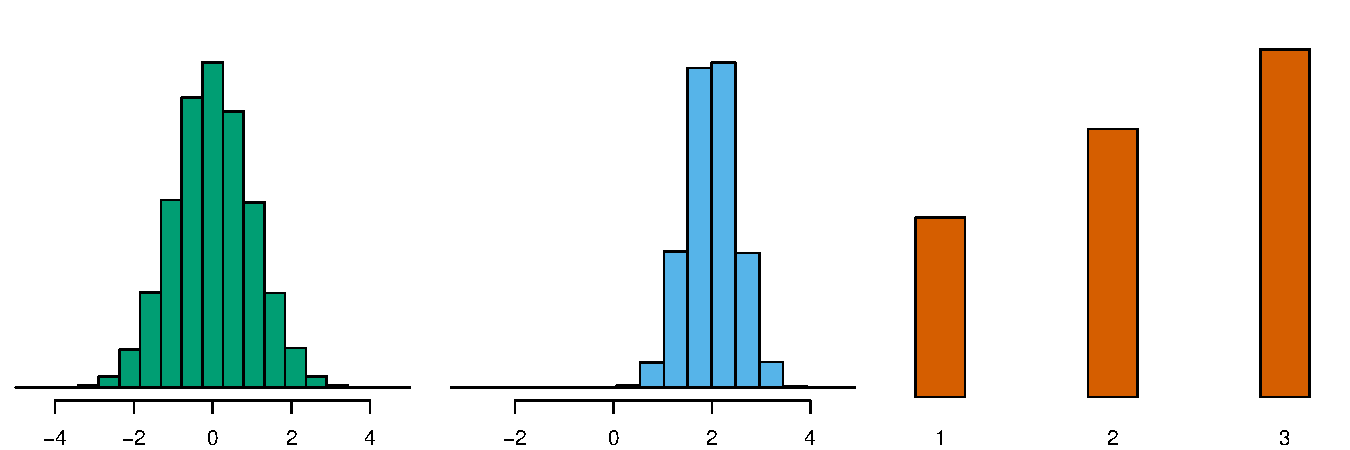
\includegraphics[width=0.80\textwidth,height=0.46\textheight,keepaspectratio]{4_10a.pdf}
  \end{center}
  \begin{takeaway}
    Test error per scenario: \emph{no classifier wins everywhere} --- the
    best method in each panel matches its data-generating process. This
    is why we compare candidates by held-out error.
  \end{takeaway}
  \islpsource{Figure 4.10}
\end{frame}

% ---------------- Extended Exercise 4.4 ----------------
\begin{frame}{Extended Exercise 4.4 \textemdash{} Choosing a classifier: three cases [Integrative]}
\begin{longexercise}
For each dataset, pick the most appropriate classifier from
\{logistic regression, LDA, QDA, naive Bayes, KNN\} and justify it in
terms of boundary shape, $n$ vs.\ $p$, within-class normality, feature
type, and number of classes.
\begin{description}
  \item[A. Credit scoring.] $n=30{,}000$ applicants, $p=6$ continuous
        predictors, $K=2$. The log-odds of default look approximately
        linear; the two classes have similar spread; income is heavily
        right-skewed.
  \item[B. Tumour diagnosis.] $n=200$ patients, $p=3$ continuous features
        that are roughly Gaussian within each class, $K=2$
        (benign / malignant). The malignant class is visibly more
        variable than the benign class.
  \item[C. Spam filtering.] $n=1{,}000$ e-mails, $p=5{,}000$ binary
        word-presence indicators, $K=2$. Features are discrete and many
        are correlated; $p\gg n$.
\end{description}
Recommend a method for each and name your runner-up.
\end{longexercise}
\end{frame}

\begin{frame}{Solution \textemdash{} Extended Exercise 4.4 (1/2)}
\begin{solutionbox}
\textbf{A quick decision checklist.}
Boundary linear? $\to$ logistic / LDA. Curved? $\to$ QDA / KNN.
Gaussian within class with equal covariance? $\to$ LDA; unequal? $\to$
QDA. $p\gg n$ or discrete features? $\to$ naive Bayes (or regularised
logistic). Highly nonlinear, large $n$, standardised continuous? $\to$
KNN.

\vspace{1mm}
\textbf{A --- Credit scoring $\Rightarrow$ logistic regression.}
Large $n$, small $p$, binary response, and an approximately linear
log-odds make logistic regression the natural first choice. It assumes
nothing about the distribution of $X$, so the skewed income variable is
harmless, and its coefficients are interpretable on the odds scale.
\emph{Runner-up:} LDA (fine under approximate normality and equal
covariance) --- but the skew makes logistic safer.

\vspace{1mm}
\textbf{B --- Tumour diagnosis $\Rightarrow$ QDA.}
Features are roughly Gaussian within class, but the covariances clearly
\emph{differ}, so the optimal boundary is quadratic --- exactly QDA's
model. With $p=3$ each class covariance has only $6$ free entries, and
$n=200$ easily supports two of them, so QDA's extra variance is
affordable. \emph{Runner-up:} LDA (its lower variance would win if $n$
were much smaller).
\end{solutionbox}
\end{frame}

\begin{frame}{Solution \textemdash{} Extended Exercise 4.4 (2/2)}
\begin{solutionbox}
\textbf{C --- Spam filtering $\Rightarrow$ naive Bayes.}
With $p=5{,}000\gg n=1{,}000$, LDA/QDA cannot estimate a $p\times p$
covariance (singular, millions of entries) and unregularised logistic
regression would overfit badly. The features are binary, not Gaussian.
Naive Bayes assumes conditional independence, needs only one-dimensional
marginals, has very low variance, and is the classic strong text
baseline. \emph{Runner-up:} $L_1/L_2$-regularised logistic regression.

\vspace{1mm}
\textbf{Where the remaining methods fit.}
\begin{itemize}
  \item \textbf{LDA} is the pick when features are Gaussian with a shared
        covariance --- a middle ground between logistic and QDA; it is the
        closest call in scenario A.
  \item \textbf{KNN} wins only when the boundary is highly nonlinear,
        the features are continuous and standardised, and $n$ is large
        relative to $p$. None of A--C qualifies; C is catastrophic for
        KNN (curse of dimensionality at $p=5{,}000$).
\end{itemize}
\begin{takeaway}
Match the method to the boundary shape, the $n$-vs-$p$ budget, and the
feature type --- then confirm the choice with held-out AUC.
\end{takeaway}
\end{solutionbox}
\end{frame}

% ============================================================
\section{Evaluation}
% ============================================================
\subsection{Confusion matrix}

\begin{frame}{Why we need more than ``accuracy''}
  Imagine a fraud detector with $99\,\%$ accuracy on a stream where
  $1\,\%$ of transactions are fraudulent.
  \begin{alertblock}{The trivial classifier}
    The model that simply \emph{always predicts ``no fraud''} has
    accuracy $99\,\%$ --- and detects zero fraud.
  \end{alertblock}
  \begin{takeaway}
    Accuracy alone is uninformative on imbalanced data. We need to
    decompose it into the four cells of a \emph{confusion matrix}.
  \end{takeaway}
\end{frame}

\begin{frame}{The confusion matrix}
  After choosing a threshold (default $0.5$), tabulate predicted vs.\
  actual:
  \begin{center}
  \begin{tabular}{l|cc|c}
    \toprule
    & Pred.\ neg.\ & Pred.\ pos.\ & Total \\
    \midrule
    True neg.\ & TN & FP & N \\
    True pos.\ & FN & TP & P \\
    \midrule
    Total & N$^*$ & P$^*$ & n \\
    \bottomrule
  \end{tabular}
  \end{center}
  \begin{readme}
    \begin{itemize}
      \item Sensitivity / recall: $\mathrm{TP}/(\mathrm{TP+FN})$ ---
            of true positives, how many did we catch?
      \item Specificity: $\mathrm{TN}/(\mathrm{TN+FP})$ --- of true
            negatives, how many did we correctly leave alone?
      \item Precision: $\mathrm{TP}/(\mathrm{TP+FP})$ --- of those we
            flagged, how many were truly positive?
    \end{itemize}
  \end{readme}
\end{frame}

\begin{frame}{The confusion matrix as a picture}
  \begin{center}
    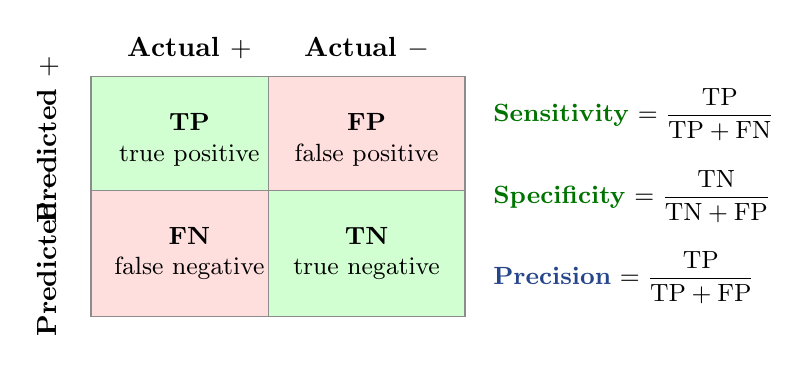
\begin{tikzpicture}[scale=0.9,font=\small,
        cell/.style={minimum width=2.5cm,minimum height=1.6cm,draw=black!45,align=center}]
      \node[font=\bfseries] at (1.25,3.0) {Actual $+$};
      \node[font=\bfseries] at (3.75,3.0) {Actual $-$};
      \node[rotate=90,font=\bfseries] at (-0.75,1.7) {Predicted $+$};
      \node[rotate=90,font=\bfseries] at (-0.75,0.1) {Predicted $-$};
      \node[cell,fill=green!18] at (1.25,1.7) {\textbf{TP}\\true positive};
      \node[cell,fill=red!13]   at (3.75,1.7) {\textbf{FP}\\false positive};
      \node[cell,fill=red!13]   at (1.25,0.1) {\textbf{FN}\\false negative};
      \node[cell,fill=green!18] at (3.75,0.1) {\textbf{TN}\\true negative};
      \node[anchor=west] at (5.4,2.05)
        {\textcolor{green!45!black}{\textbf{Sensitivity}} $=\dfrac{\mathrm{TP}}{\mathrm{TP+FN}}$};
      \node[anchor=west] at (5.4,0.9)
        {\textcolor{green!45!black}{\textbf{Specificity}} $=\dfrac{\mathrm{TN}}{\mathrm{TN+FP}}$};
      \node[anchor=west] at (5.4,-0.25)
        {\textcolor{accent}{\textbf{Precision}} $=\dfrac{\mathrm{TP}}{\mathrm{TP+FP}}$};
    \end{tikzpicture}
  \end{center}
  \begin{takeaway}
    Green cells are correct decisions, red cells are the two error types.
    Sensitivity reads down the true-positive column; specificity down the
    true-negative column; precision across the predicted-positive row.
  \end{takeaway}
\end{frame}


% ---------------- Exercise 4.8 ----------------
\begin{frame}{Exercise 4.8 \textemdash{} Reading a confusion matrix [Concept]}
\begin{exercise}
LDA on the Default data ($n=10{,}000$) with threshold $0.5$ gives:
\begin{center}\small
\begin{tabular}{l|cc|c}
\toprule
 & Pred.\ No & Pred.\ Yes & Total \\
\midrule
True No  & 9644 & 23 & 9667 \\
True Yes & 252  & 81 & 333 \\
\midrule
Total & 9896 & 104 & 10000 \\
\bottomrule
\end{tabular}
\end{center}
Compute (a) the accuracy and error rate, (b) sensitivity/recall,
(c) specificity, (d) precision. (e) Given that only $3.3\%$ of
customers default, comment on how good this classifier really is.
\end{exercise}
\end{frame}

\begin{frame}{Solution \textemdash{} Exercise 4.8 (1/2)}
\begin{solutionbox}
\textbf{Method.} First pin down the four cells --- every metric is a
ratio of them:
$\mathrm{TN}=9644$, $\mathrm{FP}=23$, $\mathrm{FN}=252$,
$\mathrm{TP}=81$, with $P=333$ actual defaulters and $N=9667$ actual
non-defaulters.

\vspace{1mm}
\textbf{(a) Accuracy} $=\dfrac{9644+81}{10000}=\dfrac{9725}{10000}
=0.9725$; error rate $=1-0.9725=2.75\%$.

\textbf{(b) Sensitivity} $=\dfrac{\mathrm{TP}}{P}=\dfrac{81}{333}
\approx 0.243$: of the $333$ customers who really default, the
classifier catches only $81$ and misses $252$.

\textbf{(c) Specificity} $=\dfrac{\mathrm{TN}}{N}=\dfrac{9644}{9667}
\approx 0.9976$: non-defaulters are almost never disturbed (only $23$
false alarms).

\textbf{(d) Precision} $=\dfrac{\mathrm{TP}}{\mathrm{TP+FP}}
=\dfrac{81}{104}\approx 0.779$: of the $104$ customers flagged, $81$
truly default.
\end{solutionbox}
\end{frame}

\begin{frame}{Solution \textemdash{} Exercise 4.8 (2/2)}
\begin{solutionbox}
\textbf{(e) Interpretation.}
The trivial classifier that \emph{always predicts ``No''} has an error
rate of $333/10000=3.33\%$ --- barely worse than LDA's $2.75\%$. So
almost all of the headline accuracy comes from the $96.7\%$ base rate
of non-defaulters, not from skill. The
high accuracy hides a poor sensitivity: LDA \emph{misses
$252/333=75.7\%$ of actual defaulters}. For a bank a missed defaulter
(FN) is the expensive kind of error,
which motivates lowering the classification threshold --- the subject
of the next exercise.

\vspace{1mm}
\textbf{Takeaway.} On imbalanced data always report the pair
(sensitivity, specificity) --- accuracy alone can be matched by a
classifier that does nothing.

\vspace{1mm}
\emph{Common mistake: mixing up sensitivity and precision. Both have
TP on top, but sensitivity divides by the \emph{actual} positives
($\mathrm{TP+FN}=333$) while precision divides by the \emph{predicted}
positives ($\mathrm{TP+FP}=104$) --- here $24.3\%$ vs.\ $77.9\%$, a
huge difference.}
\end{solutionbox}
\end{frame}

\subsection{ROC and AUC}

\begin{frame}{Why a single threshold is not enough}
  Predicting ``positive'' at $\hat p > 0.5$ is only \emph{one} operating
  point; any threshold $t$ trades sensitivity vs.\ specificity:
  \vspace{-1mm}
  \begin{center}
    
\includegraphics[width=0.84\textwidth,height=0.40\textheight,keepaspectratio]{ch04_x_threshold.png}
  \end{center}
  \vspace{-2mm}
  \begin{takeaway}
    Lower $t$ $\Rightarrow$ more true positives (sensitivity $\uparrow$)
    but more false alarms (specificity $\downarrow$); raise $t$ for the
    reverse. Choose $t$ by the cost of a false negative vs.\ a false
    positive --- a cancer screen lowers it, a spam filter raises it.
  \end{takeaway}
\end{frame}

\begin{frame}{The ROC curve}
  \begin{center}
    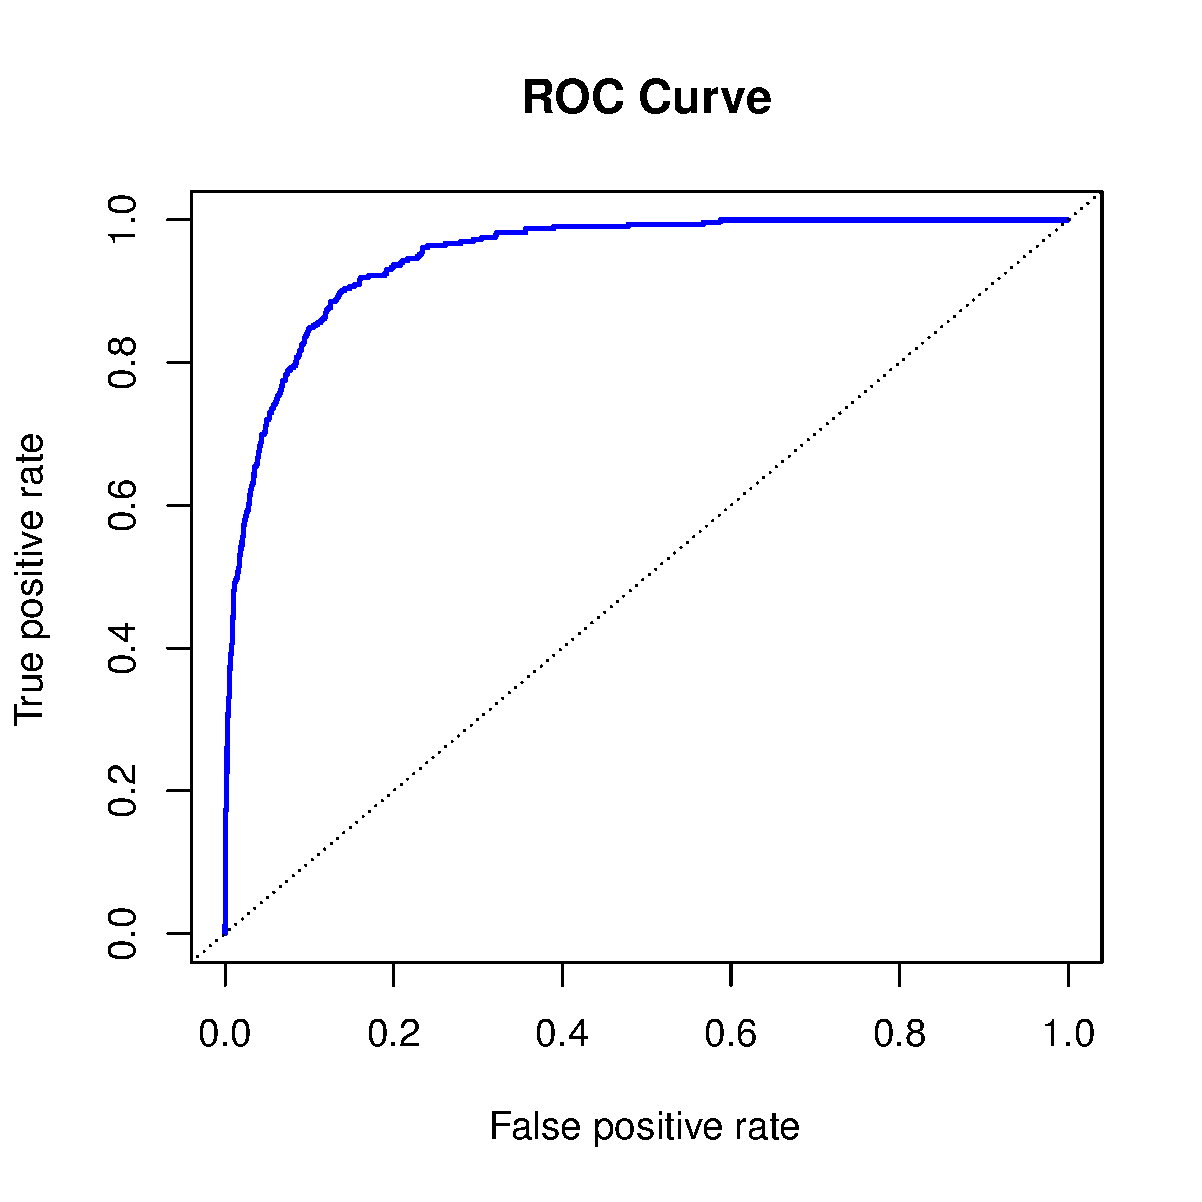
\includegraphics[width=0.50\textwidth,height=0.46\textheight,keepaspectratio]{4_8.pdf}
  \end{center}
  \begin{readme}
    $y$-axis $=$ sensitivity (true-positive rate); $x$-axis $=1-$
    specificity (false-positive rate). Each point is \emph{one}
    threshold; the $45^\circ$ diagonal is random guessing --- top-left is
    better.
  \end{readme}
  \islpsource{Figure 4.8}
\end{frame}

\begin{frame}{ROC and AUC on the Default data}
  \begin{center}
    
\includegraphics[width=0.88\textwidth,height=0.55\textheight,keepaspectratio]{ch04_roc.png}
  \end{center}
  \begin{takeaway}
    A high AUC means the model ranks defaulters above non-defaulters. The
    default $0.5$ cutoff sits low on the curve; lowering it trades
    specificity for sensitivity.
  \end{takeaway}
\end{frame}

\begin{frame}{AUC: area under the ROC curve}
  \begin{block}{Probabilistic interpretation}
    AUC $= \Pr\bigl(\hat p_+(\text{positive}) > \hat p_+(\text{negative})\bigr)$
    for a randomly chosen positive--negative pair.
  \end{block}
  \begin{readme}
    \begin{itemize}
      \item AUC $= 0.5$: model is no better than random.
      \item AUC $= 1$: perfect ranking of positives above negatives.
      \item Threshold-free summary; widely used in medicine and
            credit scoring.
    \end{itemize}
  \end{readme}
  \begin{alertblock}{Caveat under heavy class imbalance}
    AUC can look misleadingly good when one class is rare. Use
    precision-recall curves or balanced accuracy in that regime.
  \end{alertblock}
\end{frame}


% ============================================================

% ---------------- Exercise 4.9 ----------------
\begin{frame}{Exercise 4.9 \textemdash{} Threshold, ROC and AUC [Concept]}
\begin{exercise}
Lowering the LDA threshold to $0.2$ on the same Default data gives:
\begin{center}\small
\begin{tabular}{l|cc|c}
\toprule
 & Pred.\ No & Pred.\ Yes & Total \\
\midrule
True No  & 9432 & 235 & 9667 \\
True Yes & 138  & 195 & 333 \\
\bottomrule
\end{tabular}
\end{center}
\begin{enumerate}
  \item Compute sensitivity and specificity at threshold $0.2$ and
        compare with the $0.5$ results (Exercise 4.8).
  \item Compute the overall error rate at $0.2$.
  \item On ROC axes (sensitivity vs.\ $1-$specificity), how does the
        operating point move as the threshold drops from $0.5$ to $0.2$?
  \item State the probabilistic meaning of the AUC and why it is
        threshold-free.
\end{enumerate}
\end{exercise}
\end{frame}

\begin{frame}{Solution \textemdash{} Exercise 4.9 (1/2)}
\begin{solutionbox}
\textbf{Method.} Same model, same data --- only the cutoff moved, so we
recompute the two rates from the new cell counts
($\mathrm{TN}=9432$, $\mathrm{FP}=235$, $\mathrm{FN}=138$,
$\mathrm{TP}=195$) and compare operating points.

\vspace{1mm}
\textbf{(1) At threshold $0.2$.}
Sensitivity $=\dfrac{\mathrm{TP}}{\mathrm{TP+FN}}=\dfrac{195}{333}
\approx 0.586$; specificity
$=\dfrac{\mathrm{TN}}{\mathrm{TN+FP}}=\dfrac{9432}{9667}\approx 0.9757$.
Compared with $0.5$ (Exercise 4.8): sensitivity
rises from $24.3\%$ to $58.6\%$ ($81\to195$ defaulters caught), while
specificity falls from $99.76\%$ to $97.57\%$ ($23\to235$ false
alarms).

\vspace{1mm}
\textbf{(2) Error rate} $=\dfrac{\mathrm{FP+FN}}{n}
=\dfrac{235+138}{10000}=\dfrac{373}{10000}
=3.73\%$ (up from $2.75\%$) --- yet arguably the \emph{better} bank
decision, because the errors it now makes are the cheap kind.
\end{solutionbox}
\end{frame}

\begin{frame}{Solution \textemdash{} Exercise 4.9 (2/2)}
\begin{solutionbox}
\textbf{(3) ROC movement.}
With $y=$ sensitivity and $x=1-$specificity:
\[
  x:\ 1-0.9976=0.0024 \;\to\; 1-0.9757=0.0243, \qquad
  y:\ 0.243 \;\to\; 0.586 .
\]
The operating point moves \emph{up and to the right along the same ROC
curve}: a small loss of specificity buys a large gain in sensitivity.
The curve itself is fixed --- it belongs to the model's ranking, and
each threshold merely picks a point on it.

\vspace{1mm}
\textbf{(4) AUC.}
AUC $=\Pr\big(\hat p(\text{a random positive}) >
\hat p(\text{a random negative})\big)$: the probability the model ranks
a random defaulter above a random non-defaulter. It integrates over
\emph{all} thresholds, so it summarises ranking quality independently of
any single cutoff --- $0.5$ is random guessing, $1$ is a perfect
ranking.

\vspace{1mm}
\emph{Common mistake: expecting the AUC to improve after lowering the
threshold. Threshold changes slide the operating point \emph{along} the
curve; they can never move the curve --- only a better model can.}
\end{solutionbox}
\end{frame}

% ---------------- Extended Exercise 4.5 ----------------
\begin{frame}{Extended Exercise 4.5 \textemdash{} Default: logistic, confusion, ROC/AUC [Python]}
\begin{longexercise}
Using \texttt{Default.csv}:
\begin{enumerate}
  \item Fit a logistic regression of \texttt{default} on \texttt{balance},
        \texttt{income} and a $0/1$ \texttt{student} indicator
        (scikit-learn).
  \item Build the confusion matrix at thresholds $0.5$ and $0.2$.
  \item At each threshold compute accuracy, sensitivity, specificity and
        precision.
  \item Plot the ROC curve, report the AUC, and interpret the whole
        picture.
\end{enumerate}
Write runnable code and state the numbers you expect.
\end{longexercise}
\end{frame}

\begin{frame}[fragile]{Solution \textemdash{} Extended Exercise 4.5 (1/3)}
\begin{solutionbox}
\begin{lstlisting}
import pandas as pd                                  # data handling
from sklearn.linear_model import LogisticRegression  # classifier
from sklearn.metrics import (confusion_matrix, roc_auc_score,
                             RocCurveDisplay)        # evaluation tools
import matplotlib.pyplot as plt                      # plotting

df = pd.read_csv("../../ALL CSV FILES - 2nd Edition/Default.csv")  # load
y  = (df["default"] == "Yes").astype(int)          # encode response as 0/1
df["stud"] = (df["student"] == "Yes").astype(int)  # dummy-code student
X  = df[["balance", "income", "stud"]].values      # predictor matrix

clf   = LogisticRegression(max_iter=10000).fit(X, y)  # fit model (MLE)
proba = clf.predict_proba(X)[:, 1]  # predicted P(default=Yes) per customer
\end{lstlisting}
\end{solutionbox}
\end{frame}

\begin{frame}[fragile]{Solution \textemdash{} Extended Exercise 4.5 (2/3)}
\begin{solutionbox}
\begin{lstlisting}
for t in (0.5, 0.2):                       # two decision thresholds
    tn, fp, fn, tp = confusion_matrix(y, proba > t).ravel()  # cell counts
    sens, spec = tp/(tp+fn), tn/(tn+fp)    # sensitivity, specificity
    prec, acc  = tp/(tp+fp), (tp+tn)/len(y)  # precision, accuracy
    print(t, tn, fp, fn, tp,               # report all metrics
          round(acc,3), round(sens,3), round(spec,3), round(prec,3))

print("AUC =", round(roc_auc_score(y, proba), 3))  # threshold-free AUC
RocCurveDisplay.from_predictions(y, proba); plt.show()  # draw ROC curve
\end{lstlisting}
\textbf{Expected} (counts close to):
\begin{center}\scriptsize
\begin{tabular}{ccccccccc}
\toprule
$t$ & TN & FP & FN & TP & acc & sens & spec & prec\\
\midrule
0.5 & 9627 & 40  & 228 & 105 & .973 & .315 & .996 & .724\\
0.2 & 9390 & 277 & 130 & 203 & .959 & .610 & .971 & .423\\
\bottomrule
\end{tabular}
\end{center}
\vspace{-1mm}
AUC $\approx 0.950$ --- ranking quality, unchanged by the threshold.
\end{solutionbox}
\end{frame}

\begin{frame}{Solution \textemdash{} Extended Exercise 4.5 (3/3)}
\begin{solutionbox}
\textbf{Interpretation.}
\begin{itemize}
  \item \textbf{Threshold $0.5$.} Accuracy is high ($97.3\%$) but
        sensitivity is only $31.5\%$: the model misses about two-thirds of
        true defaulters. Precision is decent ($72\%$) only because it
        flags very few customers --- the always-predict-``No'' trap on
        imbalanced data.
  \item \textbf{Threshold $0.2$.} Sensitivity nearly doubles (to $61\%$),
        catching far more defaulters, at the cost of specificity
        ($99.6\%\!\to\!97.1\%$) and precision ($72\%\!\to\!42\%$): more
        false alarms. Accuracy dips slightly --- but accuracy is the wrong
        yardstick here.
  \item \textbf{ROC / AUC.} AUC $\approx 0.95$ summarises ranking quality
        over \emph{all} thresholds: a random defaulter outscores a random
        non-defaulter about $95\%$ of the time. The $0.5$ and $0.2$
        cut-offs are two operating points on the \emph{same} ROC curve, so
        the AUC does not change with the threshold.
\end{itemize}
Choose the operating point by the bank's relative cost of a missed
defaulter (FN) versus a false alarm (FP). Note \texttt{sklearn} orders the
matrix as $[[\mathrm{TN},\mathrm{FP}],[\mathrm{FN},\mathrm{TP}]]$.
\end{solutionbox}
\end{frame}

\section{GLMs}
% ============================================================

\begin{frame}{The GLM framework: one umbrella}
  Linear, logistic, and Poisson regression are all special cases of:
  \begin{block}{Generalised linear model}
    \[
      g\bigl(E[Y \mid X]\bigr) = \beta_0 + \beta_1 X_1 + \cdots + \beta_p X_p,
    \]
    where $g$ is the \emph{link function}.
  \end{block}
  \vspace{-2mm}
  \begin{center}\small
  \begin{tabular}{lll}
    \toprule
    Distribution & Link & Use \\
    \midrule
    Gaussian   & identity   & continuous $Y$ (Ch.~3) \\
    Bernoulli  & logit      & binary $Y$ (this chapter) \\
    Poisson    & log        & counts \\
    Gamma      & inverse / log & positive continuous \\
    \bottomrule
  \end{tabular}
  \end{center}
  \vspace{-2mm}
  \begin{readme}
    The \emph{link} $g$ puts the mean $E[Y\mid X]$ on a scale where a
    linear model fits; invert $g$ to predict on the original scale.
    Maximum likelihood fits the whole family.
  \end{readme}
\end{frame}

\begin{frame}{Poisson regression for counts}
  \begin{block}{Model}
    $Y \mid X \sim \mathrm{Poisson}\bigl(\lambda(X)\bigr)$ with
    $\log \lambda(X) = \beta_0 + \boldsymbol\beta^\top X$.
  \end{block}
  \begin{readme}
    Coefficients are on the log-rate scale: $\exp(\beta_j)$ is the
    multiplicative effect on the expected count. Mean equals variance
    for Poisson; if your data shows variance much greater than the
    mean, look at negative binomial instead.
  \end{readme}
  \begin{numexample}[Bikeshare]
    The Bikeshare data records bikes rented per hour. A Poisson model
    with hour-of-day, weather, and weekday gives multiplicative
    effects: ``rush-hour increases rental rate by a factor of 4.''
  \end{numexample}
\end{frame}

\begin{frame}{Bikeshare: Poisson captures the commute rhythm}
  \begin{center}
    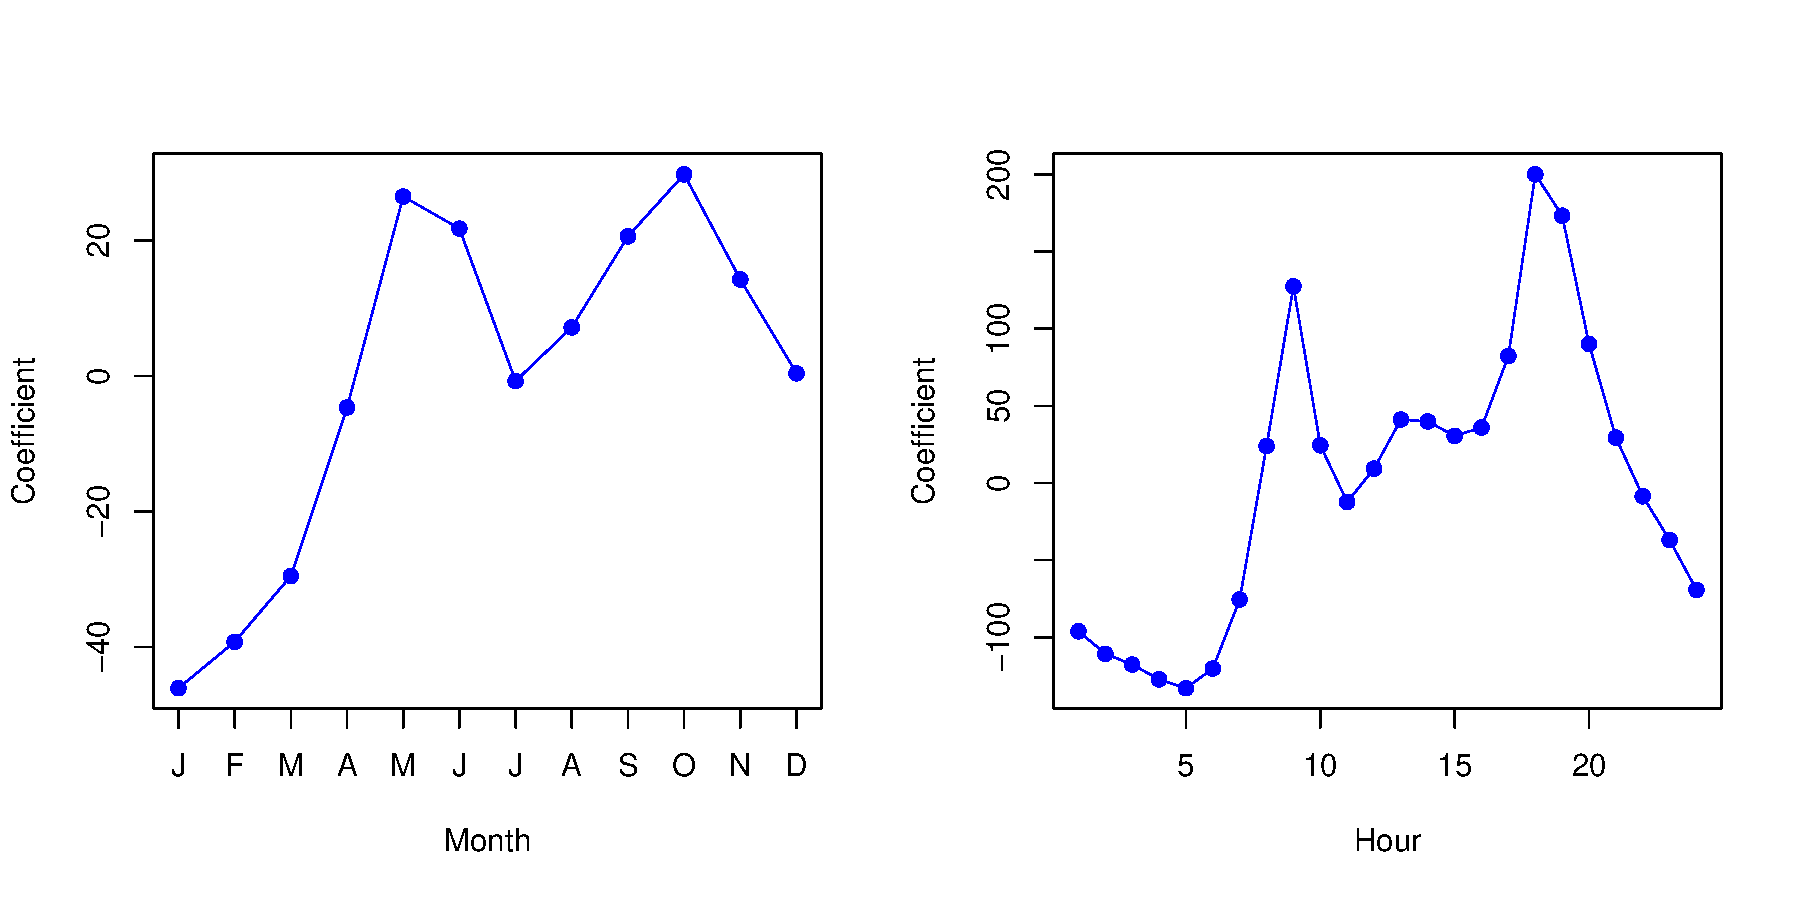
\includegraphics[width=0.80\textwidth,height=0.47\textheight,keepaspectratio]{4_13.pdf}
  \end{center}
  \begin{takeaway}
    Ridership peaks at the morning and evening commutes and climbs with
    temperature. The Poisson GLM captures these as \emph{multiplicative}
    effects on the expected count --- and never predicts a negative
    number of riders.
  \end{takeaway}
  \islpsource{Figure 4.13}
\end{frame}


% ============================================================
\section{Python Lab}

\begin{frame}{Python lab --- run it live in the notebook}
  \begin{labnote}[Companion notebook: \texttt{chapter\_04\_lab.ipynb}]
    The code in this section is meant to be \textbf{demonstrated live}. Open the companion Jupyter notebook and run it cell by cell:
    \begin{itemize}
      \item logistic regression and predicted probabilities;
      \item LDA, QDA, naive Bayes and KNN head-to-head, with ROC curves;
      \item Poisson regression on the Bikeshare data.
    \end{itemize}
    Data loads via the \texttt{ISLP} package or the bundled CSV files; the notebook ends with hands-on exercises.
  \end{labnote}
\end{frame}


% ============================================================

\begin{frame}[fragile]{Logistic regression with statsmodels}
  \begin{lstlisting}
import statsmodels.api as sm          # GLM fitting with inference
from ISLP import load_data            # textbook data loader

Default = load_data("Default")                       # load Default data
y = (Default["default"] == "Yes").astype(int)        # encode response 0/1
X = sm.add_constant(Default[["balance", "income"]])  # add intercept column

res = sm.GLM(y, X, family=sm.families.Binomial()).fit()  # logit link fit
print(res.summary())                  # coefficients, SEs, z, p-values
  \end{lstlisting}
  \texttt{statsmodels} reports each coefficient with its standard
  error, $z$-statistic, and $p$-value, plus deviance-based
  goodness-of-fit measures.
\end{frame}

\begin{frame}[fragile]{Logistic regression with scikit-learn}
  \begin{lstlisting}
from sklearn.linear_model import LogisticRegression    # classifier
from sklearn.model_selection import train_test_split   # data splitting
from sklearn.metrics import classification_report, roc_auc_score

X = Default[["balance", "income"]].values   # predictor matrix
# hold out 30% as a test set (fixed seed for reproducibility)
Xtr,Xte,ytr,yte = train_test_split(X, y, test_size=0.3, random_state=0)

lr = LogisticRegression(max_iter=1000).fit(Xtr, ytr)  # fit on training set
proba = lr.predict_proba(Xte)[:, 1]             # test-set P(default=Yes)
print(classification_report(yte, proba > 0.5))  # metrics at threshold 0.5
print("AUC:", roc_auc_score(yte, proba))        # ranking quality
  \end{lstlisting}
\end{frame}

\begin{frame}[fragile]{LDA, QDA, naive Bayes head-to-head}
  \begin{lstlisting}
from sklearn.discriminant_analysis import (
    LinearDiscriminantAnalysis    as LDA,
    QuadraticDiscriminantAnalysis as QDA)    # Gaussian discriminants
from sklearn.naive_bayes import GaussianNB   # naive Bayes (Gaussian)

for name, mdl in [("LDA", LDA()),
                  ("QDA", QDA()),
                  ("NB",  GaussianNB())]:    # three models, same split
    mdl.fit(Xtr, ytr)                        # estimate means/covariances
    p = mdl.predict_proba(Xte)[:, 1]         # posterior P(class 1) on test
    print(name, "AUC:", roc_auc_score(yte, p))  # compare by AUC
  \end{lstlisting}
\end{frame}

\begin{frame}[fragile]{ROC curves}
  \begin{lstlisting}
from sklearn.metrics import RocCurveDisplay   # ROC plotting helper
import matplotlib.pyplot as plt

fig, ax = plt.subplots(figsize=(5, 5))        # one axes, all curves
RocCurveDisplay.from_estimator(lr,  Xte, yte, ax=ax)   # logistic ROC
RocCurveDisplay.from_estimator(LDA().fit(Xtr,ytr), Xte, yte, ax=ax)  # LDA
RocCurveDisplay.from_estimator(QDA().fit(Xtr,ytr), Xte, yte, ax=ax)  # QDA
ax.plot([0,1], [0,1], "k--", linewidth=0.8); plt.show()  # chance line
  \end{lstlisting}
\end{frame}

\begin{frame}[fragile]{Poisson regression on Bikeshare}
  \begin{lstlisting}
Bike = load_data("Bikeshare")            # hourly bike-rental counts
X = sm.add_constant(Bike[["temp", "hum", "windspeed"]])  # add intercept
res = sm.GLM(Bike["bikers"], X,          # count response
             family=sm.families.Poisson()).fit()  # log link for counts
print(res.summary())                     # coefficients on log-rate scale
  \end{lstlisting}
  Coefficients are on the log-rate scale; \texttt{exp(coef)} gives
  the multiplicative effect on hourly ridership.
\end{frame}


% ============================================================

% ---------------- Exercise 4.10 ----------------
\begin{frame}{Exercise 4.10 \textemdash{} Logistic regression + confusion matrix in Python [Python]}
\begin{exercise}
Using \texttt{Default.csv}:
\begin{enumerate}
  \item Fit a logistic regression of \texttt{default} on
        \texttt{balance}, \texttt{income} and a $0/1$ \texttt{student}
        indicator with scikit-learn.
  \item Produce the confusion matrix at thresholds $0.5$ and $0.2$.
  \item Report the sensitivity at each threshold and interpret the
        trade-off.
\end{enumerate}
Write the code and describe the output you expect.
\end{exercise}
\end{frame}

\begin{frame}[fragile]{Solution \textemdash{} Exercise 4.10 (1/2)}
\begin{solutionbox}
\begin{lstlisting}
import pandas as pd                                  # data handling
from sklearn.linear_model import LogisticRegression  # classifier
from sklearn.metrics import confusion_matrix         # evaluation

df = pd.read_csv("../../ALL CSV FILES - 2nd Edition/Default.csv")  # load
y  = (df["default"] == "Yes").astype(int)          # encode response as 0/1
df["stud"] = (df["student"] == "Yes").astype(int)  # dummy-code student
X  = df[["balance", "income", "stud"]].values      # predictor matrix

clf   = LogisticRegression(max_iter=10000).fit(X, y)  # fit model (MLE)
proba = clf.predict_proba(X)[:, 1]  # predicted P(default=Yes) per customer
\end{lstlisting}
\end{solutionbox}
\end{frame}

\begin{frame}[fragile]{Solution \textemdash{} Exercise 4.10 (2/2)}
\begin{solutionbox}
\begin{lstlisting}
for t in (0.5, 0.2):                    # default and lowered threshold
    tn, fp, fn, tp = confusion_matrix(y, proba > t).ravel()  # cell counts
    sens = tp / (tp + fn)               # sensitivity = true-positive rate
    print(f"t={t}: TN={tn} FP={fp} FN={fn} TP={tp}  sens={sens:.3f}")
\end{lstlisting}

\textbf{Expected output} (counts close to):
\begin{lstlisting}
t=0.5: TN=9627 FP=40  FN=228 TP=105  sens=0.315
t=0.2: TN=9390 FP=277 FN=130 TP=203  sens=0.610
\end{lstlisting}

\textbf{Interpretation.} At the default threshold $0.5$ the model is
very accurate overall but has \emph{low sensitivity} (about $30\%$): it
misses most true defaulters, exactly as LDA did. Dropping the threshold
to $0.2$ roughly doubles sensitivity (to about $60\%$) by flagging more
customers, at the cost of more false positives (lower specificity). The
right threshold depends on the bank's relative cost of a missed
defaulter versus a false alarm. Note \texttt{sklearn}'s
\texttt{confusion\_matrix} orders cells as
$[[\mathrm{TN},\mathrm{FP}],[\mathrm{FN},\mathrm{TP}]]$.
\end{solutionbox}
\end{frame}

% ---------------- Extended Exercise 4.6 ----------------
\begin{frame}{Extended Exercise 4.6 \textemdash{} Predicting market direction out-of-sample [Python]}
\begin{longexercise}
Using \texttt{Weekly.csv} (weekly S\&P~500 returns 1990--2010;
\texttt{Direction} is Up / Down):
\begin{enumerate}
  \item Fit a logistic regression of \texttt{Direction} on
        \texttt{Lag1}--\texttt{Lag5} and \texttt{Volume} on the full data.
        What in-sample accuracy do you get, and what does the confusion
        matrix reveal?
  \item Do an \emph{honest} out-of-sample test: train on
        Year $\le 2008$, test on 2009--2010, using \texttt{Lag2} as the
        only predictor. Report test accuracy and the confusion matrix for
        logistic regression \emph{and} LDA.
  \item Compare with the naive ``always predict Up'' baseline and explain
        why market-direction prediction is so hard.
\end{enumerate}
Write runnable code and give the expected numbers.
\end{longexercise}
\end{frame}

\begin{frame}[fragile]{Solution \textemdash{} Extended Exercise 4.6 (1/3)}
\begin{solutionbox}
\begin{lstlisting}
import pandas as pd
from sklearn.linear_model import LogisticRegression
from sklearn.discriminant_analysis import LinearDiscriminantAnalysis as LDA
from sklearn.metrics import accuracy_score, confusion_matrix

wk = pd.read_csv("../../ALL CSV FILES - 2nd Edition/Weekly.csv")  # load
y  = (wk["Direction"] == "Up").astype(int)            # encode Up=1, Down=0
lags = ["Lag1","Lag2","Lag3","Lag4","Lag5","Volume"]  # predictor names

# (1) in-sample logistic on all predictors
full = LogisticRegression(max_iter=10000).fit(wk[lags], y)  # fit full model
print("acc:", round(full.score(wk[lags], y), 3))    # training accuracy
print(confusion_matrix(y, full.predict(wk[lags])))  # [[TN,FP],[FN,TP]]
\end{lstlisting}
\emph{Output:} \texttt{acc: 0.561}; confusion
$[[54,430],[48,557]]$ in order $[[\mathrm{TN},\mathrm{FP}],[\mathrm{FN},\mathrm{TP}]]$.
\end{solutionbox}
\end{frame}

\begin{frame}[fragile]{Solution \textemdash{} Extended Exercise 4.6 (2/3)}
\begin{solutionbox}
\begin{lstlisting}
# (2) train Year<=2008, test 2009-2010, using Lag2 only
tr, te = wk["Year"] <= 2008, wk["Year"] >= 2009    # boolean masks
for nm, mdl in [("logit", LogisticRegression(max_iter=10000)),
                ("LDA", LDA())]:                   # two linear classifiers
    mdl.fit(wk.loc[tr, ["Lag2"]], y[tr])           # fit on training years
    pred = mdl.predict(wk.loc[te, ["Lag2"]])       # 0/1 test predictions
    print(nm, round(accuracy_score(y[te], pred), 3),
          confusion_matrix(y[te], pred).ravel())   # acc and TN FP FN TP
\end{lstlisting}
\emph{Output:}\ \ \texttt{logit 0.625 [ 9 34 5 56]}\quad
\texttt{LDA 0.625 [ 9 34 5 56]}\ (TN FP FN TP). Both linear classifiers
give the \emph{same} result on the 2009--2010 hold-out ($n=104$).
\end{solutionbox}
\end{frame}

\begin{frame}{Solution \textemdash{} Extended Exercise 4.6 (3/3)}
\begin{solutionbox}
\textbf{Reading it.}
\begin{itemize}
  \item The full-data model reaches only $56\%$, and its confusion matrix
        shows it predicts ``Up'' almost always ($430+557$ of $1089$): the
        apparent edge is mostly the market's upward drift, not skill ---
        and this is optimistic, being in-sample.
  \item Out-of-sample (2009--2010) logistic regression and LDA give the
        \emph{same} $62.5\%$ and confusion matrix (near-identical linear
        classifiers). Both still predict ``Up'' almost every week, catching
        $56/61$ up-weeks (sensitivity $0.92$) but only $9/43$ down-weeks
        (specificity $0.21$).
  \item \textbf{Baseline.} ``Always predict Up'' already scores
        $61/104=58.7\%$; the models beat it only marginally.
\end{itemize}
\textbf{Why it is hard.} Weekly returns are close to a random walk: the
lagged predictors carry almost no signal, the signal-to-noise ratio is
tiny, and any real pattern is arbitraged away (market efficiency). Barely
beating the ``always Up'' baseline --- and only by riding the drift --- is
no basis for trading once transaction costs are included.
\end{solutionbox}
\end{frame}

\section{Summary}
% ============================================================

\begin{frame}{Chapter 4 in one slide}
  \begin{block}{What we accomplished}
    A complete classification toolkit: discriminative (logistic),
    generative (LDA / QDA / naive Bayes), evaluation (ROC, AUC), and
    the unified GLM view.
  \end{block}
  \begin{itemize}
    \item Modelled $\Pr(Y = k \mid X)$ in three different ways.
    \item Used Bayes' theorem to derive LDA and QDA.
    \item Evaluated classifiers via confusion matrices, ROC, AUC.
    \item Generalised to count data via Poisson regression.
  \end{itemize}
\end{frame}

\begin{frame}{Vocabulary checklist}
  \footnotesize
  \begin{tabular}{ll}
    \toprule
    \textbf{Term} & \textbf{Meaning} \\
    \midrule
    Logit / log-odds & $\log[p / (1 - p)]$ \\
    Maximum likelihood & Choose $\beta$ to maximise $\Pr(\mathrm{data} \mid \beta)$ \\
    Discriminative model & Models $\Pr(Y \mid X)$ directly \\
    Generative model & Models $\pi_k$ and $f_k(X)$, applies Bayes \\
    LDA / QDA & Linear / quadratic discriminant analysis \\
    Naive Bayes & Class-conditional independence assumption \\
    Sensitivity / specificity & TP/(TP+FN) / TN/(TN+FP) \\
    Precision & TP/(TP+FP) \\
    ROC / AUC & TPR vs.\ FPR / area under that curve \\
    GLM / link function & Family of regression-style models / $g(E[Y])$ \\
    \bottomrule
  \end{tabular}
\end{frame}

\begin{frame}{Key formulas at a glance}
  \begin{block}{Logistic regression}
    \[
      p(X) = \frac{e^{\beta_0 + \beta^\top X}}{1 + e^{\beta_0 + \beta^\top X}},
      \qquad
      \log\frac{p}{1-p} = \beta_0 + \beta^\top X.
    \]
  \end{block}
  \begin{block}{LDA / QDA}
    \[
      \delta_k(x) = x^\top \Sigma^{-1}\mu_k - \tfrac12 \mu_k^\top \Sigma^{-1}\mu_k + \log\pi_k.
    \]
    QDA replaces $\Sigma$ by $\Sigma_k$ and adds $-\tfrac12\log|\Sigma_k|$.
  \end{block}
  \begin{block}{Bayes posterior}
    $\Pr(Y = k \mid X) = \pi_k f_k(X) / \sum_\ell \pi_\ell f_\ell(X)$.
  \end{block}
\end{frame}

\begin{frame}{Decision rules of thumb}
  \begin{itemize}
    \item Large $n$, modest $p$, no idea about distributions
          $\Rightarrow$ logistic regression first.
    \item Small $n$, classes look Gaussian $\Rightarrow$ LDA.
    \item Many binary / categorical features, $p$ huge $\Rightarrow$
          naive Bayes.
    \item Highly nonlinear boundary, plenty of data $\Rightarrow$ try
          KNN or kernel SVM (Ch.~9).
    \item Choose the threshold by your loss function, not by default.
    \item Standardise features before fitting any distance-based model.
  \end{itemize}
\end{frame}

\begin{frame}{Common pitfalls}
  \begin{alertblock}{Don't}
    \begin{enumerate}
      \item Compare classifiers by accuracy alone on imbalanced data.
      \item Treat logistic-regression probabilities as calibrated
            without checking.
      \item Use LDA on data with obviously different class
            covariances.
      \item Forget that QDA has $K p^2/2$ parameters --- it overfits
            with small $n$.
      \item Combine LDA / QDA features without re-standardising.
      \item Ignore class priors --- in rare-event detection a
            ``perfect'' classifier with the wrong prior is unusable.
    \end{enumerate}
  \end{alertblock}
\end{frame}

\begin{frame}{Connections to the rest of the course}
  \begin{itemize}
    \item Ch.~3: linear regression is logistic regression's continuous
          twin within the GLM framework.
    \item Ch.~5: cross-validation for choosing thresholds and tuning.
    \item Ch.~6: ridge / lasso regularisation extends to logistic
          regression and GLMs.
    \item Ch.~8: tree ensembles often beat all of today's methods on
          tabular data.
    \item Ch.~9: SVMs as another linear / kernelised classifier.
    \item Ch.~10: deep learning is logistic regression with
          representation learning baked in.
  \end{itemize}
\end{frame}

\begin{frame}{Self-check questions}
  \begin{enumerate}
    \item Why does ordinary linear regression fail for binary $Y$?
    \item In the Default data, why does \texttt{student} flip sign
          once \texttt{balance} is included?
    \item Derive the LDA discriminant from Bayes' rule, assuming
          $X \mid Y = k \sim \mathcal{N}(\mu_k, \Sigma)$.
    \item When does naive Bayes outperform logistic regression even
          though its independence assumption is wrong?
    \item Sketch a confusion matrix for a fraud detector with $99\,\%$
          accuracy on data with $1\,\%$ fraud. Is it useful?
    \item Explain ROC and AUC. What does a $45^\circ$ ROC mean?
  \end{enumerate}
\end{frame}

\begin{frame}{Ten things to remember}
  \begin{enumerate}
    \item Linear regression is wrong for categorical $Y$ --- use a GLM.
    \item Logistic regression: linear in log-odds.
    \item Estimation by maximum likelihood; no closed form.
    \item LDA: Gaussian classes, common $\Sigma$ $\Rightarrow$ linear
          boundary.
    \item QDA: separate $\Sigma_k$ $\Rightarrow$ quadratic boundary.
    \item Naive Bayes: feature independence $\Rightarrow$ very low
          variance.
    \item Univariate slopes can flip sign --- watch for confounding.
    \item Confusion matrix, sensitivity, specificity, ROC, AUC.
    \item Threshold choice depends on costs.
    \item Poisson GLM for counts; same framework via the link.
  \end{enumerate}
\end{frame}

\begin{frame}{What's next}
  Chapter 5: \emph{Resampling Methods}.
  \begin{itemize}
    \item Validation set, LOOCV, $k$-fold cross-validation.
    \item The bootstrap.
    \item Why these are the most important tools in your toolbox.
  \end{itemize}
\end{frame}

\end{document}
